% ============================================================
% Tire-Road Friction Identification via ESC-Gradient and
% Burckhardt Model: Implementation, Validation, and
% Robustness Analysis
%
% Preprint — NTT DATA BEST Hackathon 2026
% Politecnico di Torino, Turin, Italy
% ============================================================

\documentclass[11pt,a4paper]{article}

% ── Packages ────────────────────────────────────────────────
\usepackage[T1]{fontenc}
\usepackage[utf8]{inputenc}
\usepackage{lmodern}
\usepackage[margin=2.5cm]{geometry}
\usepackage{amsmath,amssymb,bm}
\usepackage{graphicx}
\usepackage{booktabs}
\usepackage{xcolor}
\usepackage{hyperref}
\usepackage{cleveref}
\usepackage{microtype}
\usepackage{parskip}
\usepackage{float}
\usepackage{siunitx}
\usepackage{algorithm}
\usepackage{algpseudocode}
\usepackage[numbers,sort&compress]{natbib}
\usepackage{url}
\usepackage{lineno}

\hypersetup{
  colorlinks=true,
  linkcolor=blue!70!black,
  citecolor=green!50!black,
  urlcolor=blue!70!black,
  pdfauthor={NTT DATA Hackathon Team},
  pdftitle={Tire-Road Friction Identification via ESC-Gradient and Burckhardt Model},
}

% ── Graphics path ───────────────────────────────────────────
\graphicspath{{./plots/}}

% ── Custom commands ─────────────────────────────────────────
\newcommand{\mumax}{\mu_{\mathrm{peak}}}
\newcommand{\sopt}{s_{\mathrm{opt}}}
\newcommand{\vvec}[1]{\bm{#1}}
\newcommand{\norm}[1]{\left\lVert #1 \right\rVert}
\newcommand{\doi}[1]{\href{https://doi.org/#1}{\texttt{doi:#1}}}
% cleveref algorithm name
\crefname{algorithm}{Algorithm}{Algorithms}
\Crefname{algorithm}{Algorithm}{Algorithms}
% ── Title ───────────────────────────────────────────────────
\title{%
  \textbf{Tire-Road Friction Identification via ESC-Gradient\\
  and the Burckhardt Model: Implementation, Validation,\\
  and Robustness Analysis}\\[0.8em]
  {\large A Three-Layer Real-Time Identifier with Offline\\
  Machine-Learning Validation on Simulink Data}
}

\author{%
  NTT DATA BEST Hackathon 2026\\
  Politecnico di Torino, Turin, Italy\\[0.3em]
  \texttt{s328433@studenti.polito.it} \quad
  \texttt{s340464@studenti.polito.it}
}

\date{28 March 2026 \quad|\quad Preprint}

% ============================================================
\begin{document}
% ============================================================

\maketitle

% ── Abstract ────────────────────────────────────────────────
\begin{abstract}
Accurate real-time knowledge of the tire-road friction coefficient is critical
for vehicle safety systems including the Anti-lock Braking System~(ABS),
Electronic Stability Control~(ESC), and advanced driver-assistance systems~(ADAS).
We present the design, Python implementation, and systematic validation of a
three-layer tire-road friction identifier that combines a Lookup Table~(LUT),
an analytic ESC-gradient layer, and a Brent root-finding refinement to estimate
the Burckhardt model parameters $(c_1, c_2, c_3)$ in real time.
The identifier is validated on synthetic Simulink data generated across 48 braking
scenarios~(eight scenarios~$\times$~three brake distributions~$\times$~two modes)
covering dry asphalt, wet asphalt, and snow.
An offline machine-learning evaluation using Burckhardt nonlinear least-squares
fitting and nearest-neighbour classification achieves a macro-average
$F_1 = 1.000$ on clean simulation data;
however, we provide a rigorous analysis demonstrating that this result is
mathematically guaranteed by construction and therefore does not constitute
evidence of real-world generalisation.
A three-source realistic noise model---covering friction sensor noise
($\sigma_\mu$), slip encoder noise ($\sigma_s$), and per-run parameter drift
($\sigma_p$)---reveals that the classifier degrades to $F_1 \approx 0.58$ when
the slip range is restricted to $s < 0.05$, which corresponds to normal driving
conditions outside of active braking.
These results quantify the operating envelope of the proposed identifier and
provide a principled baseline for future validation on real experimental data.
\end{abstract}

\bigskip
\noindent\textbf{Keywords:} tire-road friction estimation; Burckhardt model; ESC gradient identifier; ABS; Brent method; Simulink; surface classification; robustness analysis.

\bigskip
% ============================================================
\section{Introduction}
\label{sec:intro}
% ============================================================

The friction coefficient between the tire contact patch and the road surface is
the fundamental scalar quantity that limits all longitudinal and lateral force
generation in a ground vehicle.
It appears directly in the force balance of every safety-critical control system:
ABS regulates wheel slip to maximise friction; ESC corrects yaw by modulating
individual wheel brakes; and advanced emergency braking systems must anticipate
stopping distances before the driver reacts~\cite{rajamani2012,pacejka2006}.

Despite its importance, the friction coefficient cannot be measured directly by
any sensor available on a production vehicle.
It must be \emph{estimated} from indirect signals---wheel speed, longitudinal
acceleration, brake pressure---under the constraint that the estimate must be
available within a single brake-control cycle (typically \SIrange{10}{20}{\milli\second}).

The standard approach to online friction estimation is to fit a parametric model
of the tire friction curve, $\mu(s)$, to measured $(s, \mu)$ data, where $s$ is
the wheel slip ratio.
Among the many parameterisations in the literature---Pacejka Magic
Formula~\cite{pacejka2006}, Dugoff~\cite{dugoff1970}, Fiala~\cite{fiala1954},
LuGre~\cite{canudas1995}---the Burckhardt model~\cite{burckhardt1993} offers a particularly favourable
trade-off between accuracy and identifiability for real-time use: it has only
three parameters, each with direct physical interpretation, and admits a
closed-form expression for the optimal slip---a property not shared by the
Pacejka Magic Formula or the LuGre model.

This paper makes the following contributions:
\begin{enumerate}
  \item A complete Python port of a MATLAB three-layer ESC-gradient Burckhardt
        identifier (\texttt{hackaton\_id.py}), reproducing the exact behaviour
        of the MATLAB persistent-state implementation.
  \item A 48-scenario Simulink validation dataset with full signal provenance,
        preprocessing pipeline, and exploratory analysis.
  \item An offline surface-classification pipeline and a rigorous evaluation of
        its limitations, including explicit identification of the circular-reasoning
        trap inherent in closed-loop simulation evaluation.
  \item A three-source realistic noise model and a systematic robustness sweep that
        characterises the operating envelope across sensor noise, slip-range limitation,
        and parameter drift.
\end{enumerate}

The remainder of the paper is organised as follows.
\Cref{sec:model} reviews the Burckhardt friction model.
\Cref{sec:identifier} describes the three-layer identifier.
\Cref{sec:data} presents the Simulink dataset and preprocessing pipeline.
\Cref{sec:offline} describes the offline machine-learning evaluation.
\Cref{sec:evaluation} presents classification and robustness results.
\Cref{sec:discussion} discusses limitations and future work.
\Cref{sec:conclusion} concludes.

% ============================================================
\section{The Burckhardt Tire Friction Model}
\label{sec:model}
% ============================================================

\subsection{Model Formulation}

The Burckhardt model~\cite{burckhardt1993} describes the longitudinal friction
coefficient as a function of the wheel slip ratio $s \in [0,1]$:
\begin{equation}
  \mu(s) = c_1 \bigl(1 - e^{-c_2 |s|}\bigr) - c_3 |s|
  \label{eq:burckhardt}
\end{equation}
where $c_1 > 0$ is the peak friction amplitude, $c_2 > 0$ is the curve sharpness
(large on ice/snow, small on dry asphalt), and $c_3 > 0$ is the descending slope
after the peak.
The model is valid for $|s| \in [0, 1]$ and produces a physical friction peak
when $c_1 c_2 > c_3$.

\subsection{Optimal Slip and Peak Friction}

Setting $\mathrm{d}\mu / \mathrm{d}|s| = 0$ gives the closed-form optimal slip:
\begin{equation}
  \sopt = \frac{1}{c_2} \ln\!\left(\frac{c_1 c_2}{c_3}\right), \qquad
  c_1 c_2 > c_3
  \label{eq:sopt}
\end{equation}
and the corresponding peak friction:
\begin{equation}
  \mumax = \mu(\sopt) = c_1\!\left(1 - e^{-c_2 \sopt}\right) - c_3 \sopt
  \label{eq:mupeak}
\end{equation}

\subsection{Surface Parameters}

\Cref{tab:surfaces} lists the nominal Burckhardt parameters for the three surfaces
used in this study, taken from \cite{burckhardt1993,rajamani2012}.
\Cref{fig:surfaces_overview} shows the corresponding friction curves.

\begin{table}[htbp]
  \centering
  \caption{Burckhardt model parameters for standard road surfaces~\cite{burckhardt1993,rajamani2012}.
           The Simulink dataset covers the first three surfaces.
           Ice is included in the offline model-comparison experiments only.}
  \label{tab:surfaces}
  \begin{tabular}{lccccc}
    \toprule
    Surface & $c_1$ & $c_2$ & $c_3$ & $\mumax$ & $\sopt$ \\
    \midrule
    Dry asphalt & 1.2801 & 23.990 & 0.5200 & 1.170 & 0.170 \\
    Wet asphalt & 0.8570 & 33.822 & 0.3470 & 0.801 & 0.131 \\
    Snow        & 0.1946 & 94.129 & 0.0646 & 0.190 & 0.060 \\
    Ice         & 0.0500 & 306.40 & 0.0010 & 0.050 & 0.027 \\
    \bottomrule
  \end{tabular}
\end{table}

\begin{figure}[htbp]
  \centering
  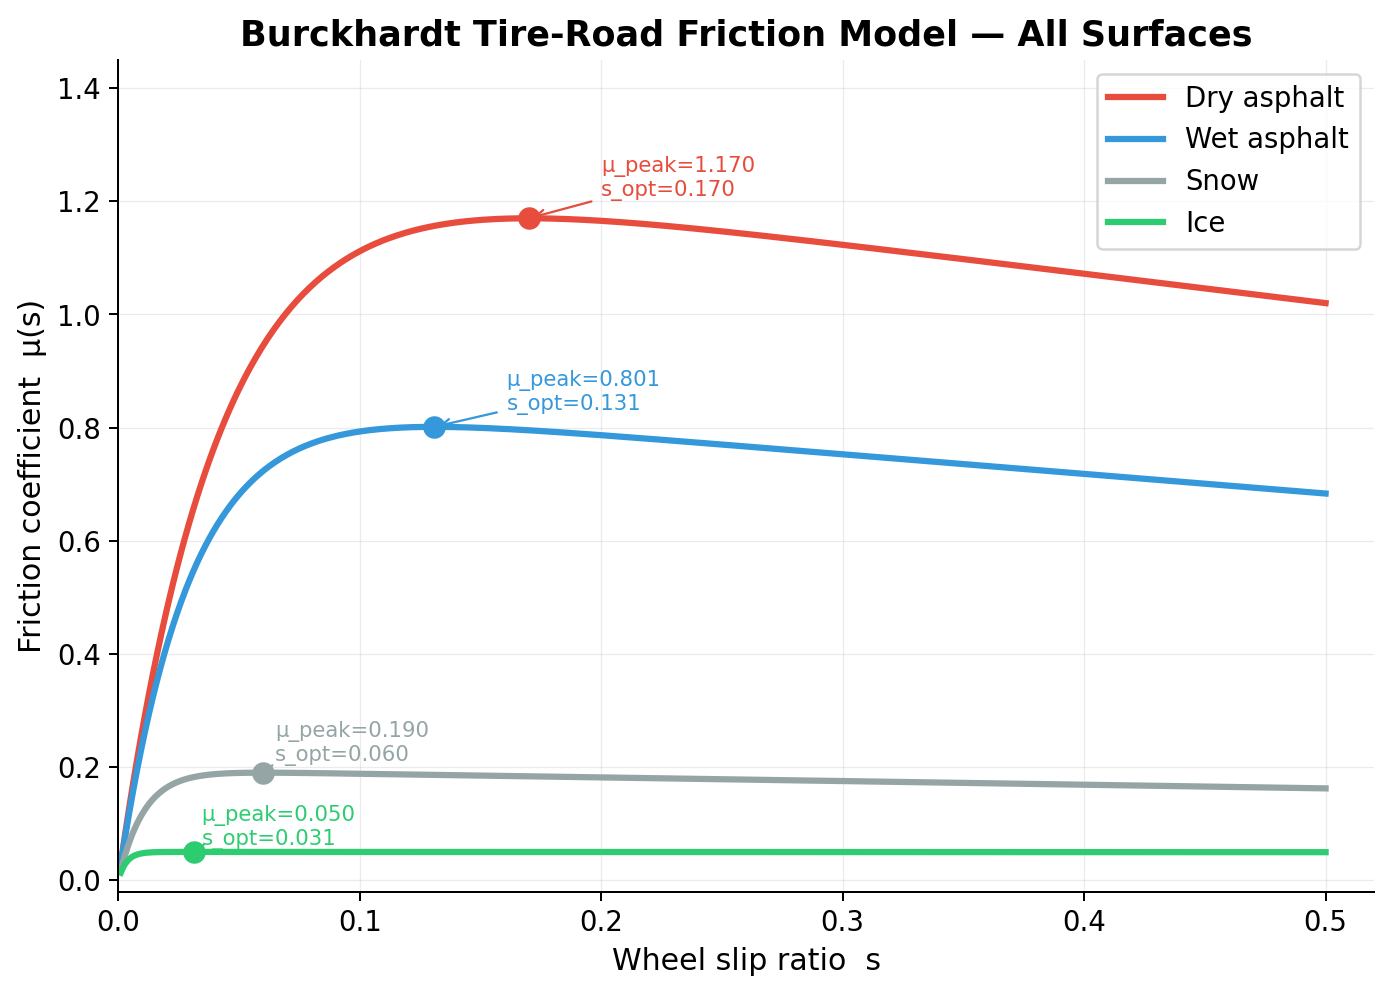
\includegraphics[width=0.75\textwidth]{01_surfaces_overview.png}
  \caption{Burckhardt friction curves for dry asphalt, wet asphalt, and snow.
           Circles mark $(\sopt, \mumax)$ for each surface.
           Note the large separation in $c_2$: 24 (dry) vs.\ 34 (wet) vs.\ 94 (snow),
           which is the primary discriminating feature for surface classification.}
  \label{fig:surfaces_overview}
\end{figure}

\subsection{Gradient of the Friction Curve}

The analytic gradient is used in Layer~2 of the identifier (\cref{sec:identifier}):
\begin{equation}
  \frac{\mathrm{d}\mu}{\mathrm{d}|s|} = c_1 c_2 e^{-c_2 |s|} - c_3
  \label{eq:gradient}
\end{equation}
At $s = \sopt$ this gradient is zero; at any other operating point it provides
additional constraints for solving the inverse problem.

% ============================================================
\section{Three-Layer ESC-Gradient Identifier}
\label{sec:identifier}
% ============================================================

\subsection{Overview}

The real-time identifier, referred to as \textsc{ESC\_TwoPoint\_ID}~v3, runs at
every timestep of the ABS/ESC controller.
It maintains persistent state across timesteps---implemented in Python as a class
with instance attributes---and produces updated estimates $(c_1, c_2, c_3)$
along with the derived quantities $\sopt$ and $\mumax$.

The identifier uses three hierarchical layers, summarised in \cref{alg:identifier}:

\begin{enumerate}
  \item \textbf{Layer~1 (LUT):} A precomputed lookup table maps the observed
        peak friction $\hat\mu_{\max}$ to a coarse estimate of $c_2$.
        This layer is always active and provides an immediate fallback-safe estimate.
  \item \textbf{Layer~2 (ESC-Gradient Analytic):} Given the ESC gradient
        $g_\mathrm{esc}$ from the outer extremum-seeking controller, the true
        friction gradient at the current operating point is recovered as
        $g_\mathrm{true} = -g_\mathrm{esc} \cdot 2 / a_\mathrm{esc}$,
        where $a_\mathrm{esc}$ is the ESC dither amplitude.
        This allows $c_1$ and $c_3$ to be solved \emph{analytically} at any
        operating point, not just at the friction peak.
  \item \textbf{Layer~3 (Brent Root-Finding):} When the ESC probe has explored
        a sufficiently wide slip range ($|s_\mathrm{probe} - s_\mathrm{peak}|
        > \delta_s$, with $\delta_s = 0.008$ in all experiments),
        a two-point root-finding problem is solved
        for $c_2$ using Brent's method~\cite{brent1973}.
\end{enumerate}

\subsection{Layer 1 --- Lookup Table}

A precomputed table maps the running maximum of observed friction
$\hat\mu_\mathrm{max}$ to a coarse estimate of $c_2$.
This provides an immediate estimate at every timestep with no iteration,
serving as both an initialisation for Layers~2 and~3 and a safe fallback
when gradient information is unavailable.
The LUT is clamped to the physical range $c_2 \in [c_{2,\min}, c_{2,\max}]$
defined by the parameter vector.

\begin{algorithm}[H]
\caption{ESC\_TwoPoint\_ID~v3 (one timestep)}
\label{alg:identifier}
\begin{algorithmic}[1]
\Require $\mu_\mathrm{meas}$, $s_\mathrm{meas}$, $s_\mathrm{probe}$,
         $g_\mathrm{esc}$, $a_\mathrm{esc}$, $t$, params,
         $(c_1^\mathrm{prev}, c_2^\mathrm{prev}, c_3^\mathrm{prev})$
\Ensure updated $(c_1, c_2, c_3, \sopt, \mumax, \mathrm{valid}, \mathrm{flag})$
\If{$t < t_\mathrm{start}$}
  \State \Return previous estimates \Comment{Layer 1: warmup}
\EndIf
\State $c_2 \leftarrow \mathrm{LUT}(\hat\mu_\mathrm{max})$ \Comment{Layer 1: LUT}
\If{$g_\mathrm{esc}$ available}
  \State $g_\mathrm{true} \leftarrow -g_\mathrm{esc} \cdot 2 / a_\mathrm{esc}$
  \State Solve analytically for $c_1, c_3$ using \cref{eq:burckhardt,eq:gradient}
         \Comment{Layer 2: ESC-gradient}
\Else
  \State Use peak-based fallback for $c_1, c_3$
\EndIf
\If{$|s_\mathrm{probe} - s_\mathrm{peak}| > \delta_s$}
  \State Solve $\mu_\mathrm{probe} = \mu(s_\mathrm{probe}; c_1(c_2), c_3(c_2))$
         for $c_2$ via Brent \Comment{Layer 3: Brent}
\EndIf
\State $\sopt \leftarrow \ln(c_1 c_2 / c_3) / c_2$
\State $\mumax \leftarrow \mu(\sopt)$
\State \Return $(c_1, c_2, c_3, \sopt, \mumax, \mathrm{valid}, \mathrm{flag})$
\end{algorithmic}
\end{algorithm}

\subsection{Layer 2 — Analytic ESC-Gradient Solution (v3 Key Innovation)}

Previous versions of the identifier (v1/v2) assumed that the buffer maximum
equals the true friction peak, i.e.\ $\mathrm{d}\mu/\mathrm{d}s = 0$.
This assumption fails whenever the ESC perturbation places the operating point
away from the peak---particularly on snow where the peak is sharp ($c_2 = 94$)
and easily overshot.

Version~3 relaxes this by exploiting the analytic gradient \cref{eq:gradient}.
At any operating point $(s_k, \mu_k)$ with known gradient $g_k$:
\begin{align}
  c_1 &= \frac{\mu_k - g_k |s_k|}{1 - (1 + c_2 |s_k|) e^{-c_2 |s_k|}}
  \label{eq:c1_analytic} \\
  c_3 &= c_1 c_2 e^{-c_2 |s_k|} - g_k
  \label{eq:c3_analytic}
\end{align}
These expressions require only a known $c_2$ (from Layer~1) and are valid for
any $s_k \neq 0$.
Note that the denominator of \cref{eq:c1_analytic} approaches zero as
$c_2|s_k| \to 0$ (L'H\^{o}pital: $\lim_{x\to 0}[1-(1+x)e^{-x}] = 0$);
the implementation enforces a minimum slip threshold of $|s_k| > 0.005$
to prevent numerical blow-up during low-slip warmup phases.
The key insight is that the ESC gradient $g_\mathrm{esc}$ is directly available
from the outer extremum-seeking controller's low-pass filter demodulator:
$g_\mathrm{esc} \approx \mathrm{LPF}[\mu \cdot \sin(\omega t)] \cdot (2/a)$.

\subsection{Layer 3 — Brent Root-Finding for $c_2$}

When the ESC has excited a sufficiently wide slip range
($|s_\mathrm{probe} - s_\mathrm{peak}| > \delta_s$),
a two-point constraint is available:
\begin{equation}
  f(c_2) = \mu_\mathrm{probe} - \mu(s_\mathrm{probe};\, c_1(c_2),\, c_3(c_2)) = 0
\end{equation}
This is solved for $c_2$ using Brent's method~\cite{brent1973}, which guarantees
superlinear convergence within a bracketed interval.
The initial bracket $[c_{2,\mathrm{LUT}} \cdot 0.5,\; c_{2,\mathrm{LUT}} \cdot 2]$
is tried first; the full physical range $[c_{2,\min}, c_{2,\max}]$ is the fallback.

\subsection{Convergence Simulation}

\Cref{fig:convergence} shows the identifier converging from an incorrect initial
guess (wet asphalt parameters) to the true surface (dry asphalt) over 300
synthetic timesteps.
All three parameters converge within approximately 1.5~s of simulation time.

\begin{figure}[htbp]
  \centering
  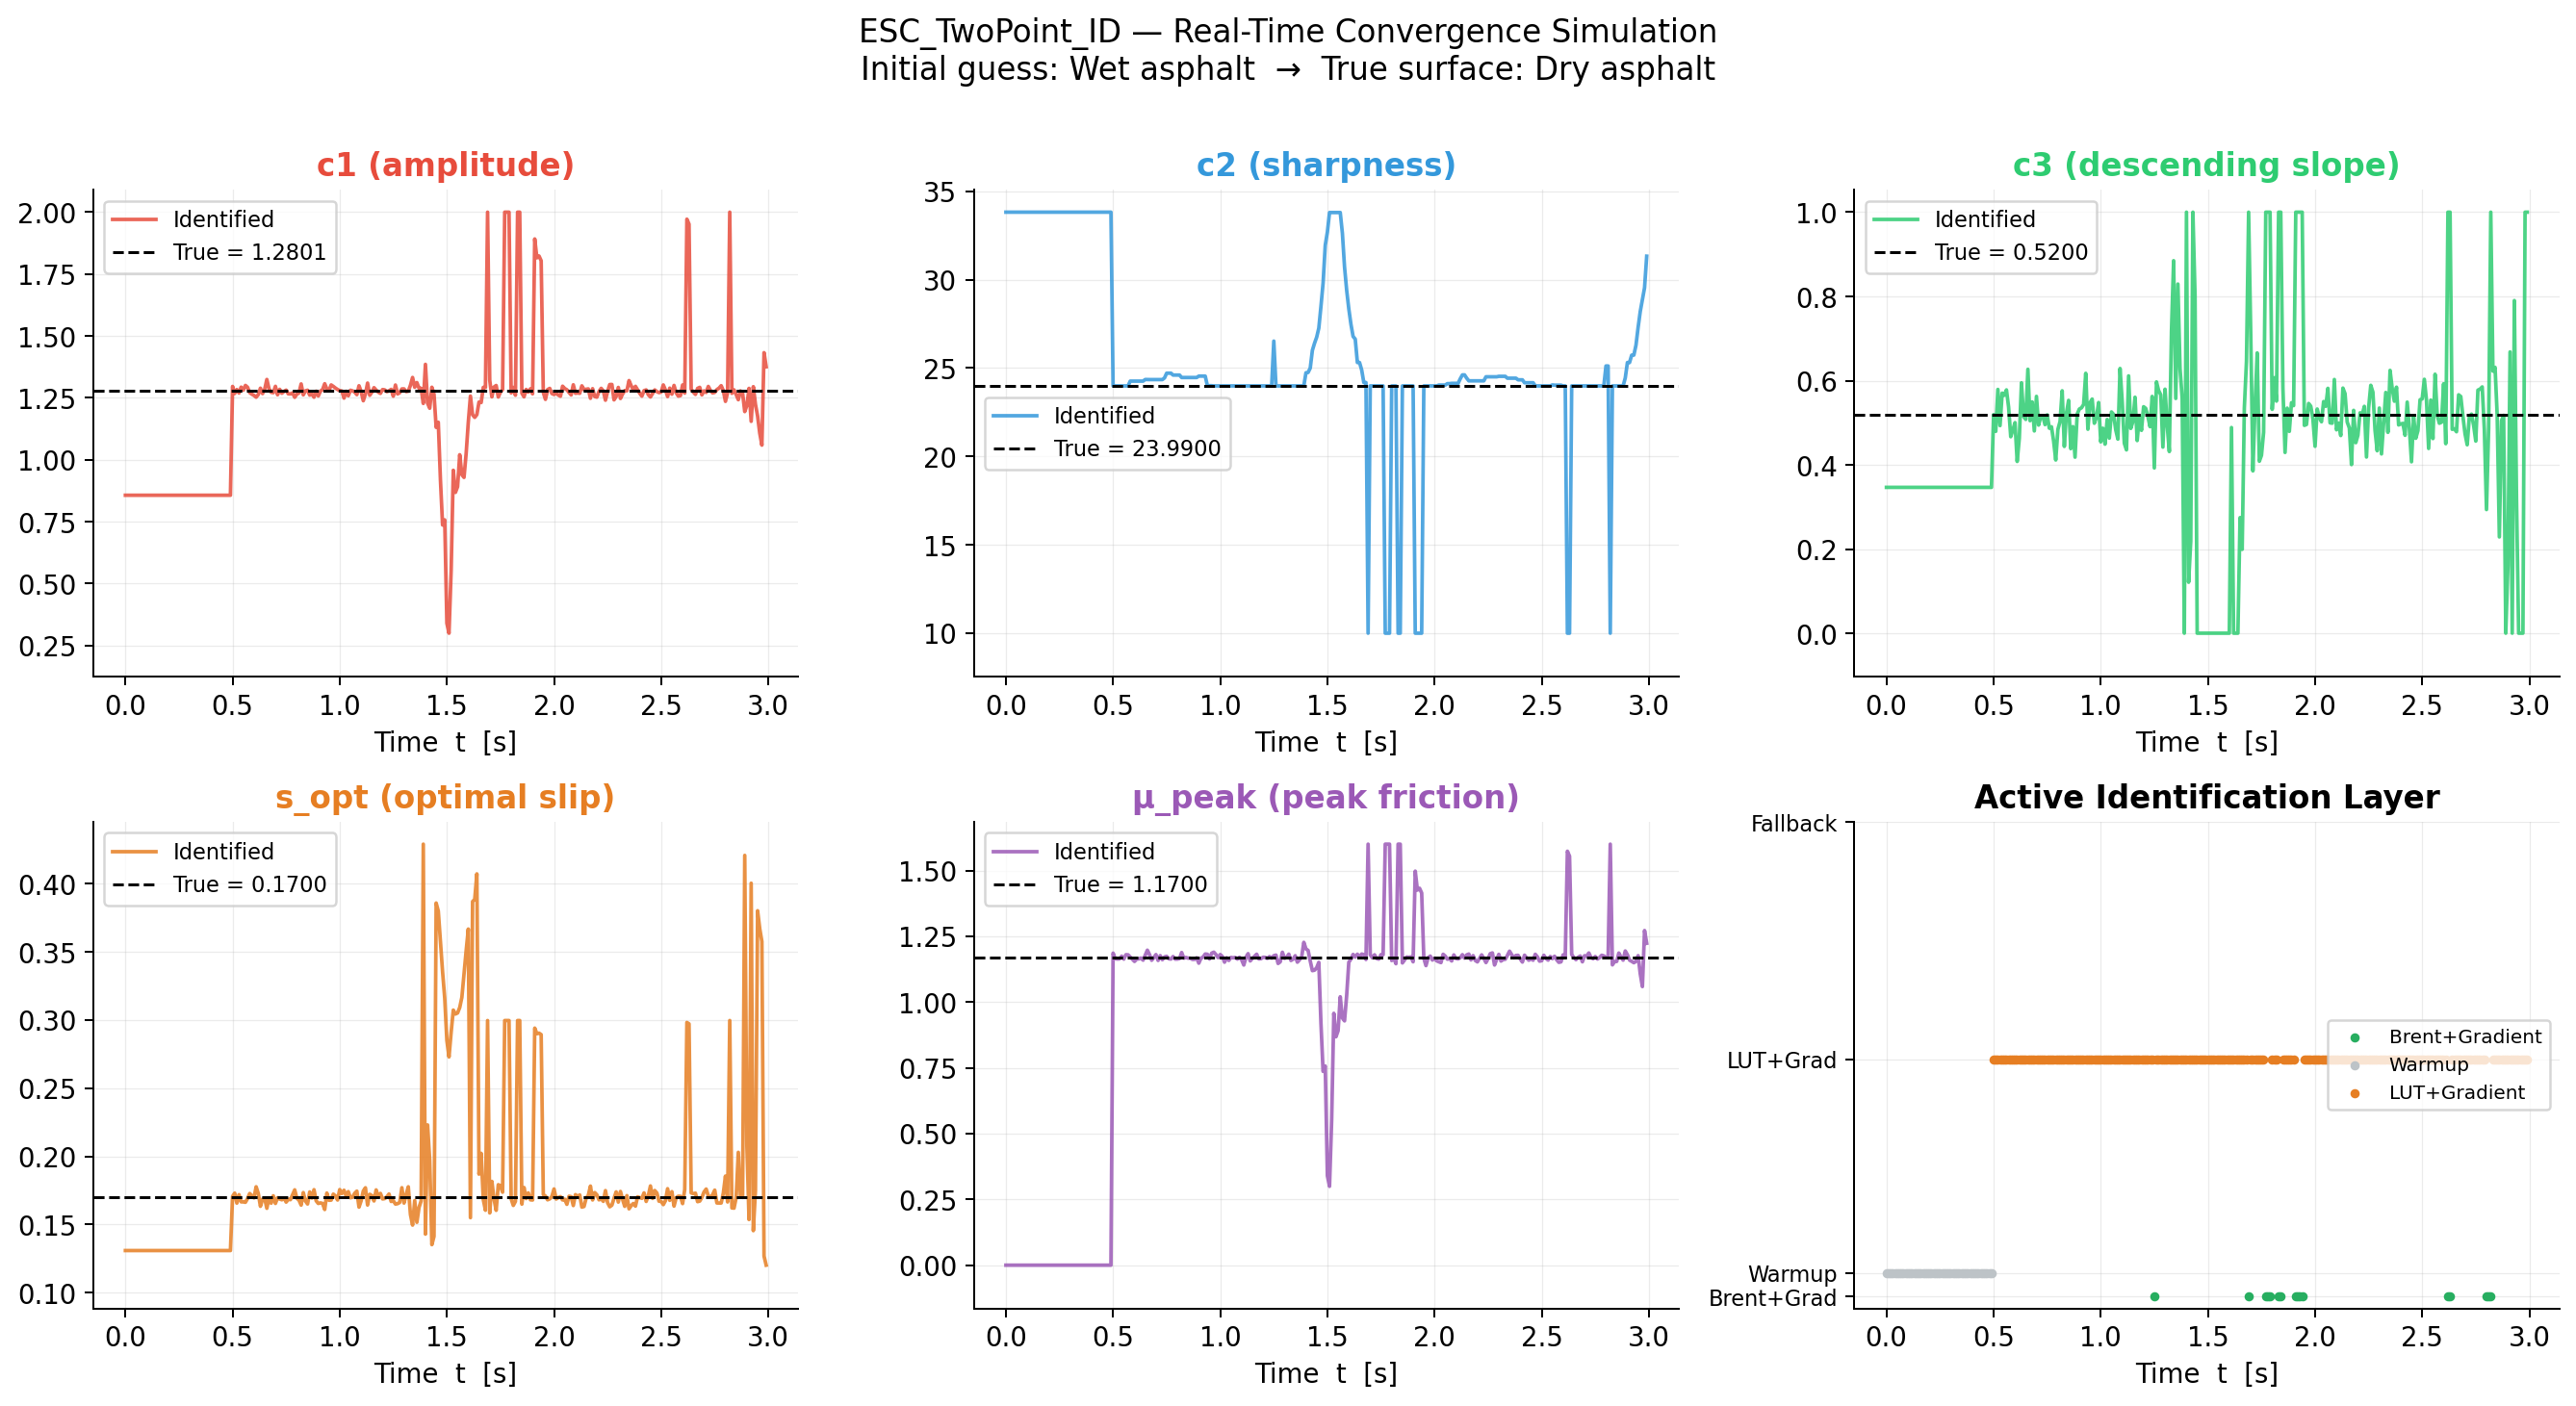
\includegraphics[width=\textwidth]{05_identifier_convergence.png}
  \caption{Simulated convergence of the three-layer ESC identifier.
           Initial surface assumption: wet asphalt ($c_1=0.857, c_2=33.8$).
           True surface: dry asphalt ($c_1=1.280, c_2=23.99$).
           Top row: parameter estimates $c_1, c_2, c_3$ vs.\ time.
           Bottom row: derived $\sopt$, $\mumax$, and active layer flag.}
  \label{fig:convergence}
\end{figure}

% ============================================================
\section{Simulation Dataset and Preprocessing}
\label{sec:data}
% ============================================================

\subsection{Simulink Simulation}

The dataset was generated using a Simulink/MATLAB vehicle dynamics model with
the ESC framework~\cite{hackatonid2026}.
A total of 48 braking scenarios were executed:
8 scenarios $\times$ 3 brake force distributions $\times$ 2 simulation modes
(\texttt{Framework}, \texttt{NoABS}).

\Cref{tab:scenarios} summarises the scenario structure.
Each scenario produces time-series signals at every wheel for all four simulation
timesteps, exported via a MATLAB script to a flat CSV with 29 columns.

\begin{table}[htbp]
  \centering
  \caption{Simulation scenario structure (48 total runs).
           Each of the 8 named scenarios (3 surfaces $\times$ Low/High braking
           on one surface + 2 combined scenarios) is run with 3 brake
           distributions and 2 modes.}
  \label{tab:scenarios}
  \begin{tabular}{llc}
    \toprule
    Dimension & Values & Count \\
    \midrule
    Named scenarios & Per-surface Low/High + combined & 8 \\
    Brake distribution & Front-biased, Balanced, Rear-biased & 3 \\
    Simulation mode & Framework (ABS on), NoABS (open-loop) & 2 \\
    \midrule
    \multicolumn{2}{l}{Total runs ($8 \times 3 \times 2$)} & \textbf{48} \\
    \bottomrule
  \end{tabular}
\end{table}

The raw CSV (\texttt{friction\_data\_full.csv}) contains 765{,}000 rows.
The primary signals are listed in \cref{tab:signals}.

\begin{table}[htbp]
  \centering
  \caption{Key signals exported from the Simulink simulation.}
  \label{tab:signals}
  \begin{tabular}{llp{7cm}}
    \toprule
    Signal & Unit & Description \\
    \midrule
    \texttt{slip} & -- & $|s_\mathrm{measured}|$, wheel slip ratio \\
    \texttt{mu\_noisy} & -- & Measured friction coefficient (sensor noise included) \\
    \texttt{alpha} & -- & Identifier confidence $\in [0,1]$ \\
    \texttt{abs\_active} & -- & 1 when ABS was controlling (alpha $> 0.001$) \\
    \texttt{g\_esc} & -- & ESC gradient estimate from LPF demodulator \\
    \texttt{c1\_true / c2\_true / c3\_true} & -- & Ground-truth Burckhardt parameters \\
    \texttt{mu\_true} & -- & Noiseless friction (ground truth) \\
    \texttt{s\_opt\_true} & -- & Ground-truth optimal slip \\
    \bottomrule
  \end{tabular}
\end{table}

\subsection{Preprocessing Pipeline}

Raw data is processed through a five-stage pipeline~(\texttt{preprocess.py}):

\begin{enumerate}
  \item \textbf{Column removal.}
        Twelve columns uninformative for friction modelling are dropped:
        \texttt{s\_hat} (100\% NaN), redundant metadata (\texttt{road\_1/2},
        \texttt{case\_no}), ESC design parameters (\texttt{dither}, \texttt{a\_esc},
        \texttt{s\_probe}), and run-level metrics (\texttt{d\_stop}, \texttt{t\_stop},
        \texttt{T\_front}, \texttt{T\_rear}).
  \item \textbf{ABS-active filter.}
        Only rows with \texttt{abs\_active}$=1$ are retained.
        Free-rolling rows (ABS inactive) contain slip values near zero that carry
        no information about the friction curve.
        This reduces the dataset from 765{,}000 to 479{,}000 rows.
  \item \textbf{Confidence filter.}
        Rows with identifier confidence $\alpha < 0.01$ are removed, eliminating
        identifier warmup transients (479{,}000 $\to$ 340{,}000 rows).
  \item \textbf{Temporal thinning.}
        Consecutive timesteps at \SI{1}{\kilo\hertz} are strongly autocorrelated.
        A stride of~10 is applied within each run$\times$wheel group
        (340{,}000 $\to$ 48{,}000 rows).
  \item \textbf{Surface balancing.}
        The raw dataset is heavily imbalanced: 82\% snow, 9\% dry, 9\% wet.
        Stratified undersampling caps snow at 12{,}000 and each other surface
        at 6{,}000 rows while preserving scenario diversity within each surface
        (48{,}000 $\to$ 20{,}616 rows).
\end{enumerate}

\Cref{fig:slip_dist,fig:scenario_coverage} show the data distributions
before and after preprocessing.

\begin{figure}[htbp]
  \centering
  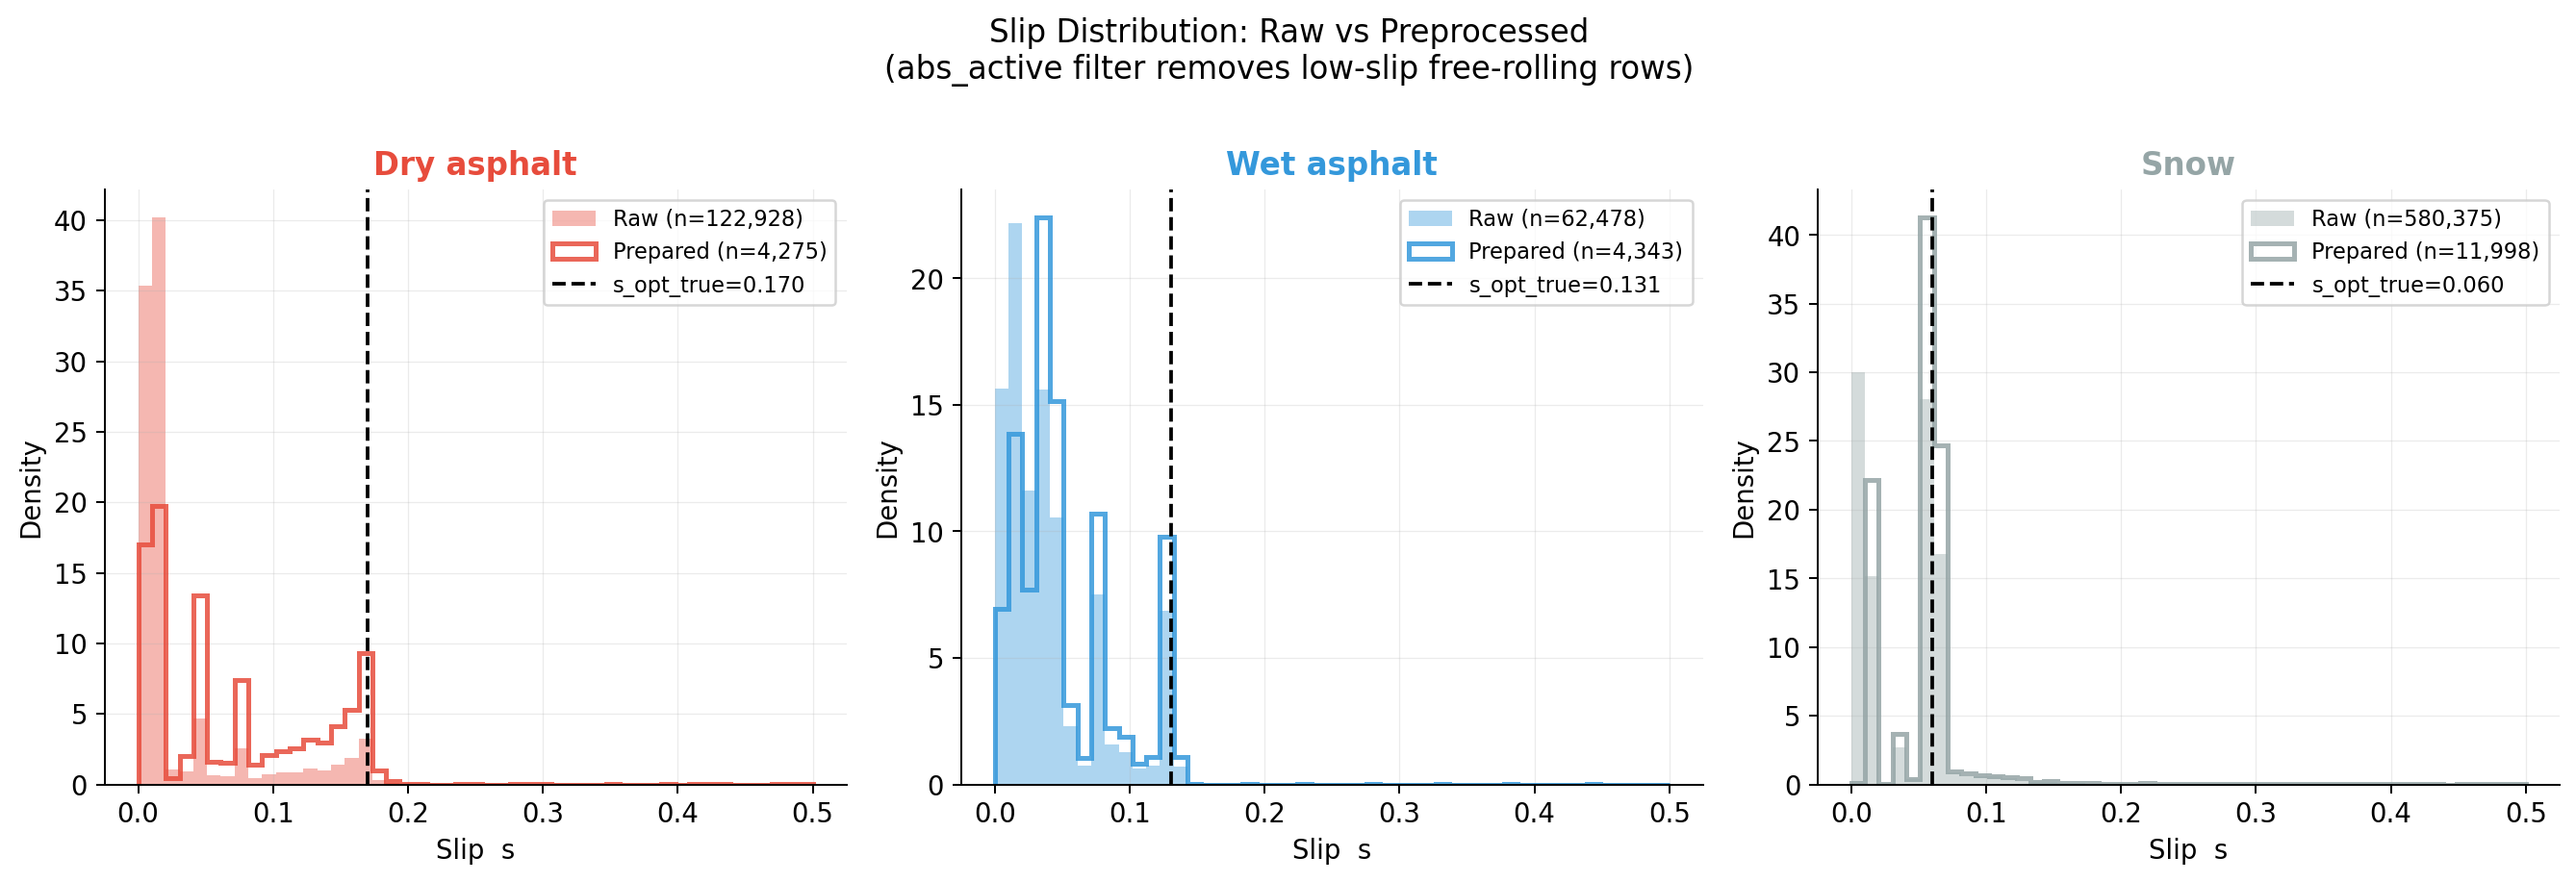
\includegraphics[width=\textwidth]{06_data_slip_distribution.png}
  \caption{Slip distributions before (raw, shaded) and after (solid outline)
           preprocessing for each surface.
           Vertical dashed lines mark the ground-truth $\sopt$ for each surface.
           The preprocessing pipeline removes low-slip free-rolling rows and
           thins autocorrelated time-series, shifting the distribution toward
           higher-information slip values.}
  \label{fig:slip_dist}
\end{figure}

\begin{figure}[htbp]
  \centering
  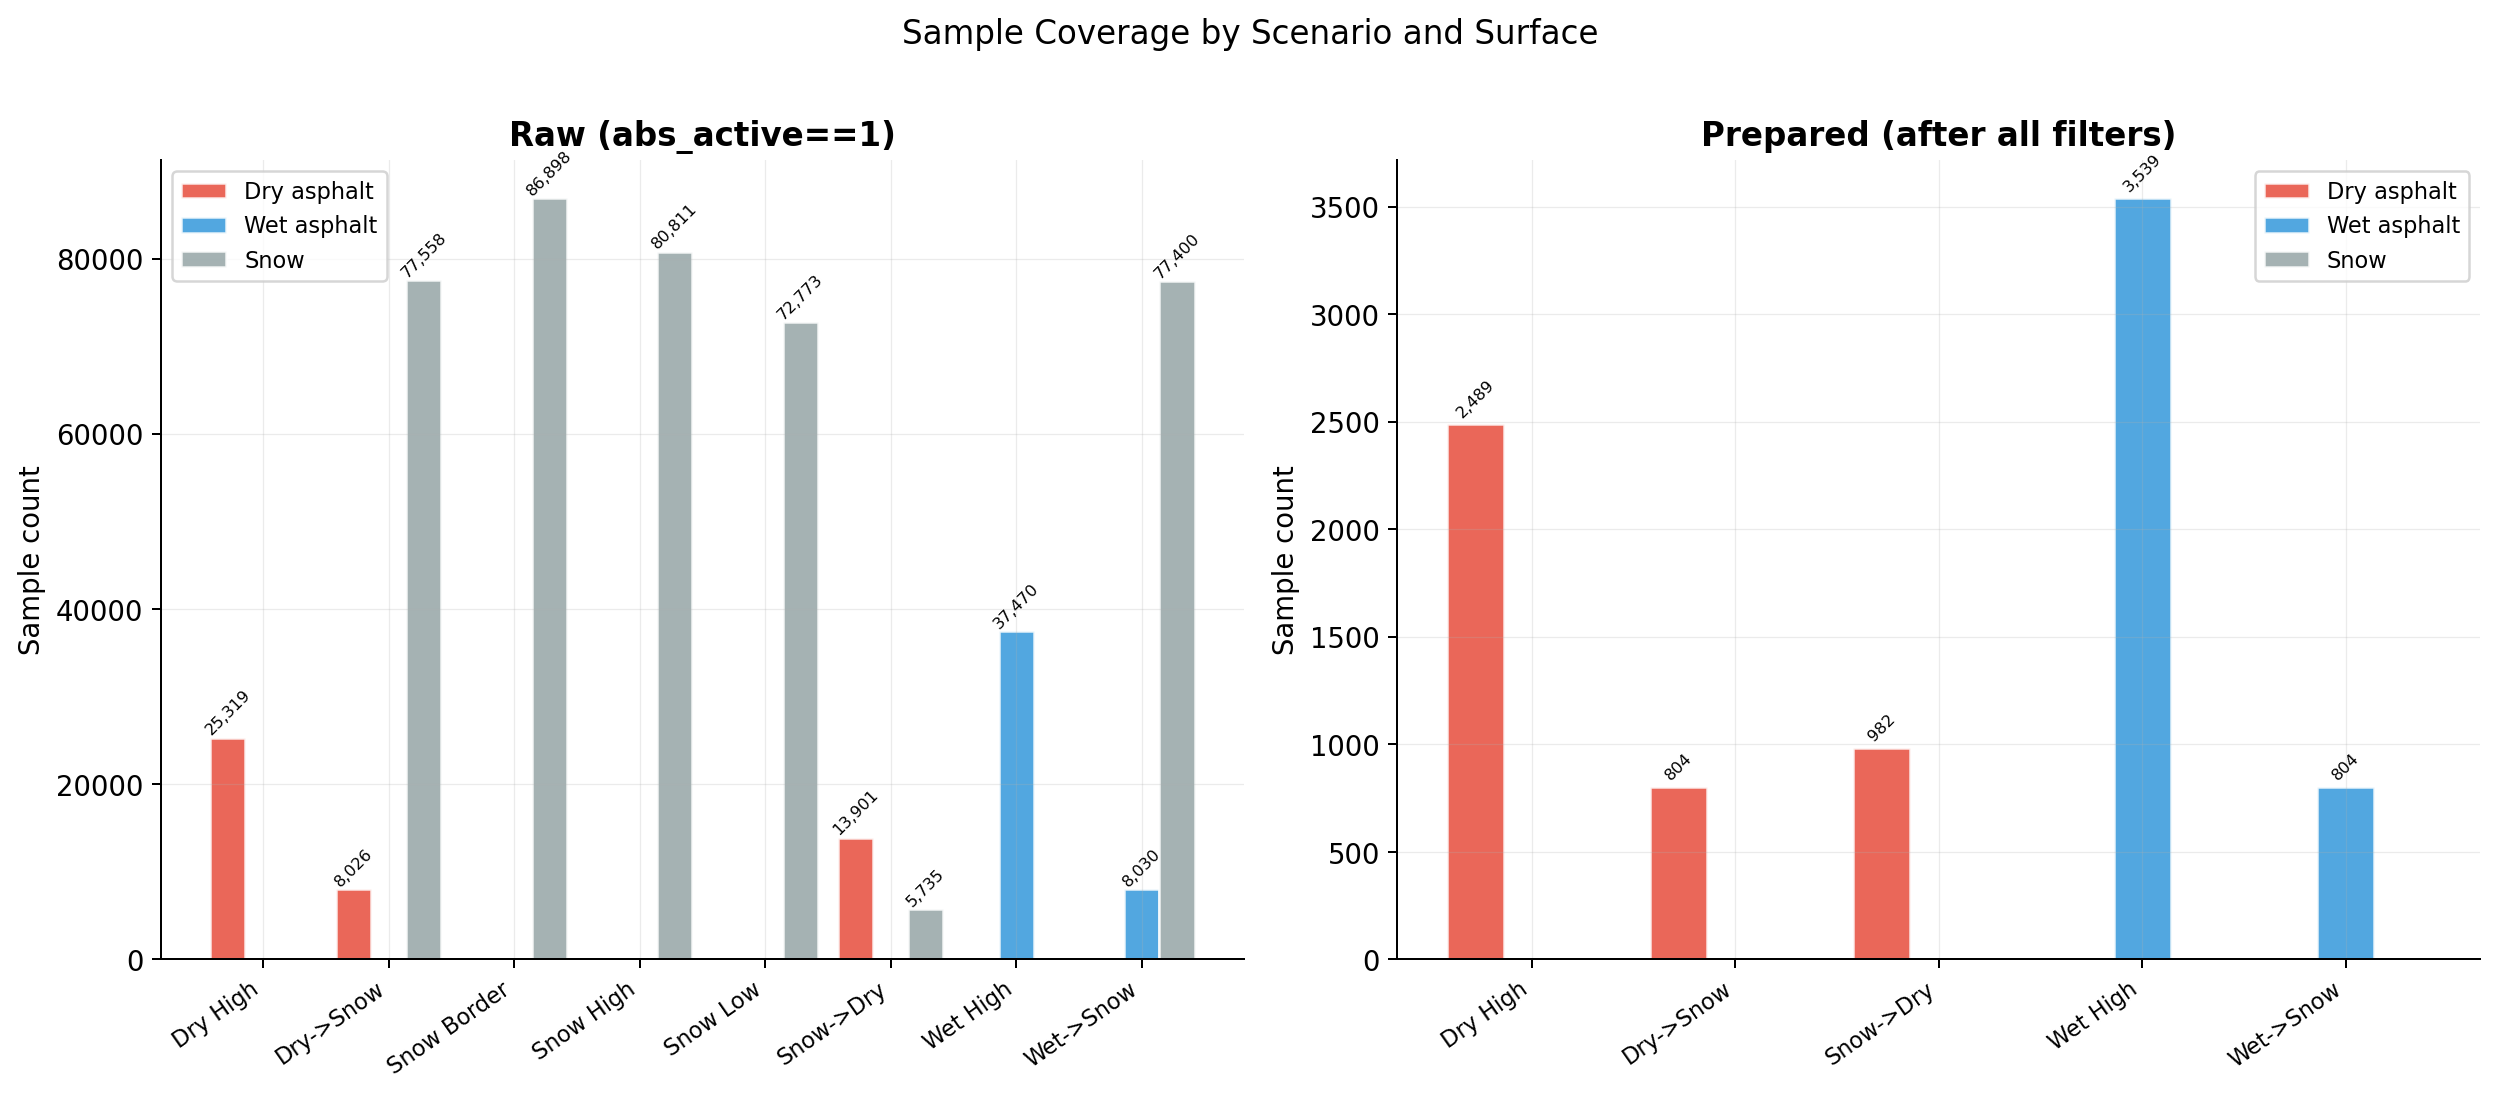
\includegraphics[width=0.9\textwidth]{09_data_scenario_coverage.png}
  \caption{Sample counts per scenario and surface, before and after preprocessing.
           Snow dominates the raw dataset (left); stratified undersampling restores
           balance (right).}
  \label{fig:scenario_coverage}
\end{figure}

\subsection{Data Quality Verification}

\Cref{fig:real_vs_model} shows the preprocessed measurements overlaid on the
ground-truth Burckhardt curves.
The residual $|\mu_\mathrm{noisy} - \mu_\mathrm{true}| < 3 \times 10^{-4}$
confirms that the simulation uses the Burckhardt model exactly, with only
numerical noise at the level of floating-point precision.
This property is essential for understanding the evaluation results in \cref{sec:evaluation}.

\begin{figure}[htbp]
  \centering
  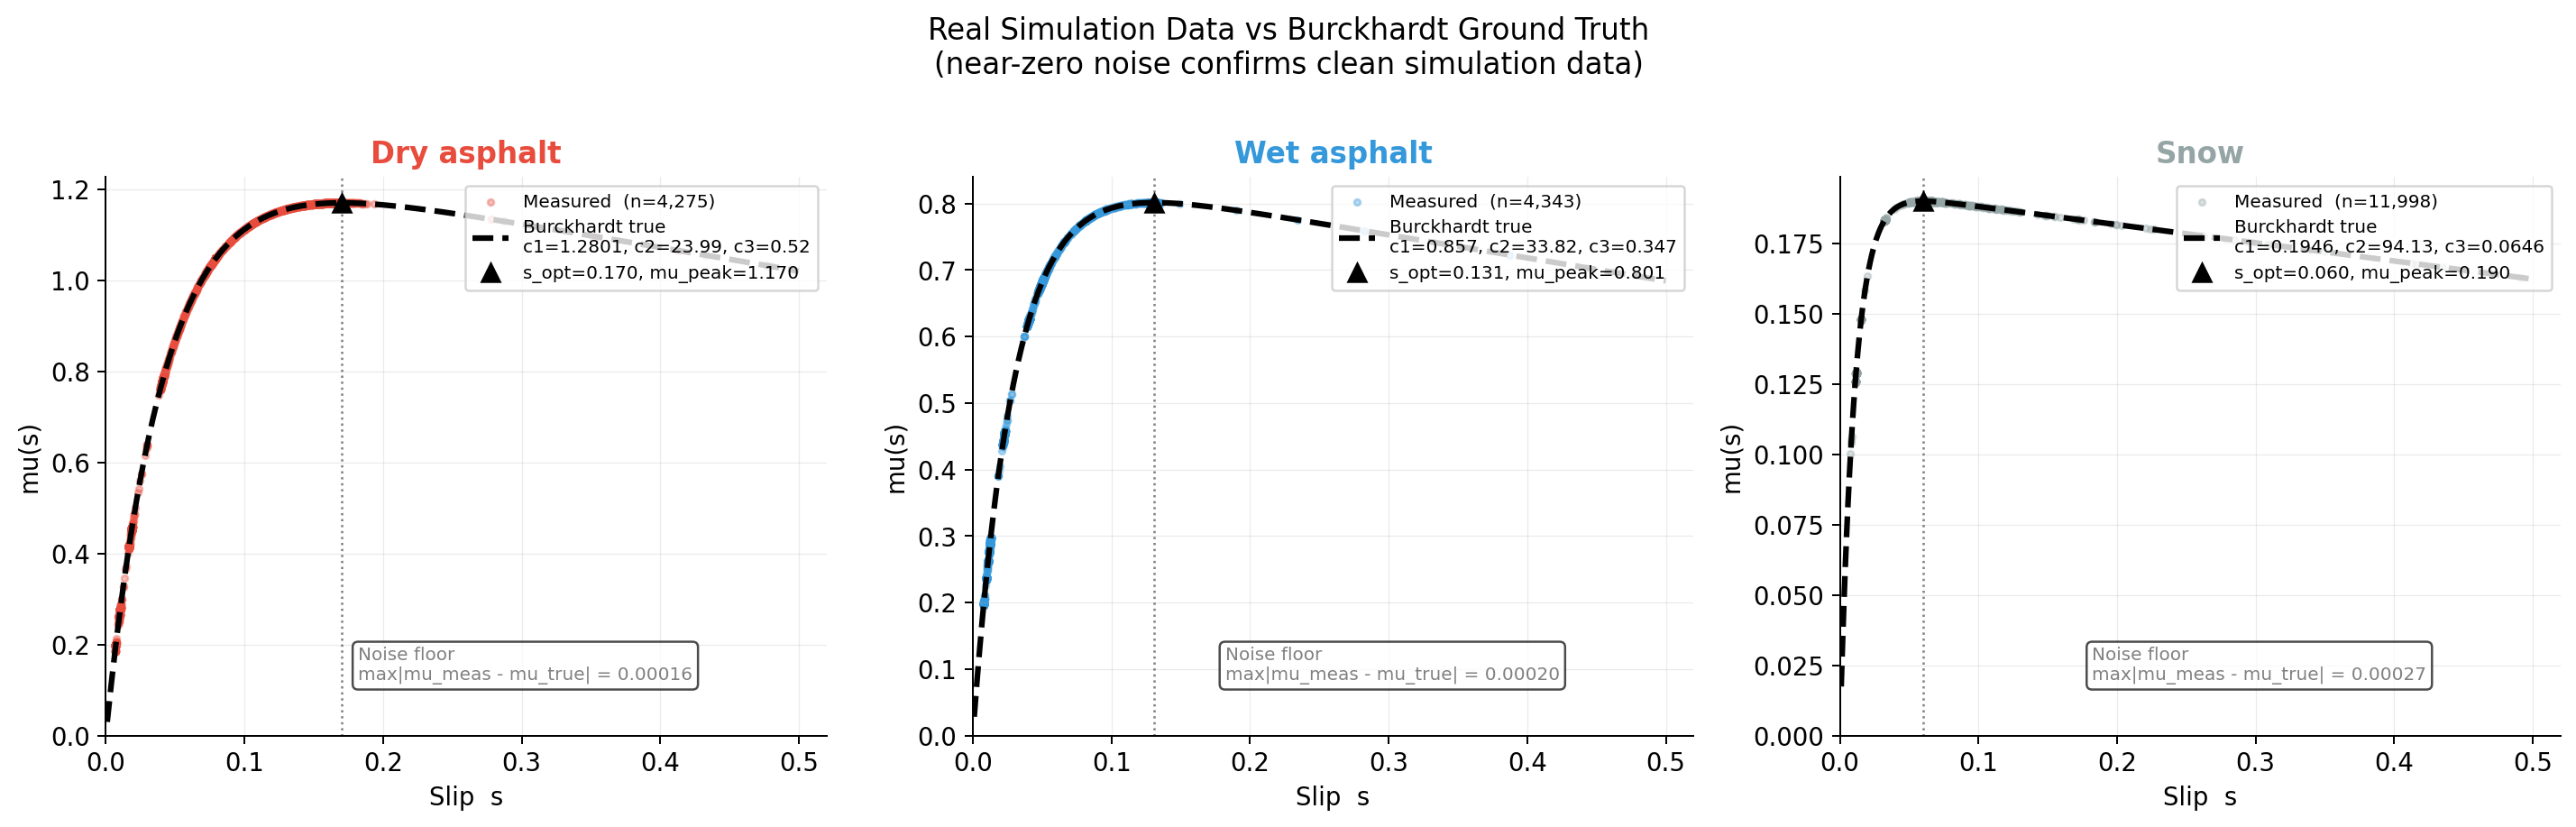
\includegraphics[width=\textwidth]{10_data_real_vs_model.png}
  \caption{Preprocessed simulation measurements (scatter) vs.\ Burckhardt
           ground-truth curves (dashed) for each surface.
           The near-zero noise floor ($<3\times10^{-4}$) confirms that the
           Simulink model applies the Burckhardt formula exactly.}
  \label{fig:real_vs_model}
\end{figure}

% ============================================================
\section{Offline Machine-Learning Evaluation}
\label{sec:offline}
% ============================================================

\subsection{Three-Model Comparison}

To validate the Burckhardt parameter estimation offline, three modelling
approaches are compared on synthetic datasets generated from the known
surface parameters~(\cref{tab:surfaces}):

\begin{description}
  \item[Burckhardt NLS] Nonlinear least-squares fitting using
        \texttt{scipy.curve\_fit} with physical parameter bounds
        $c_1 \in [0.01, 1.5]$, $c_2 \in [23, 310]$, $c_3 \in [0.001, 0.6]$.
        Three initialisations are tried; the best residual is kept.
  \item[Gaussian Process (GP)] A \texttt{sklearn} Gaussian Process Regressor with
        a squared-exponential (RBF) kernel scaled by a \texttt{ConstantKernel},
        plus a \texttt{WhiteKernel} noise floor for regularisation.
        Five random restarts of the optimiser avoid local optima.
        Outputs posterior mean and standard deviation.
  \item[Neural Network (NN)] A three-layer Multi-Layer Perceptron~(MLP) with
        architecture $(64, 64, 32)$, early stopping (patience applied to 15\%
        validation fraction), and \texttt{StandardScaler}
        normalisation on inputs and outputs.
\end{description}

\Cref{fig:model_comparison,fig:rmse_comparison} show the fitted curves and
RMSE on held-out test data for $n_\mathrm{train} = 50$ points.

\begin{figure}[htbp]
  \centering
  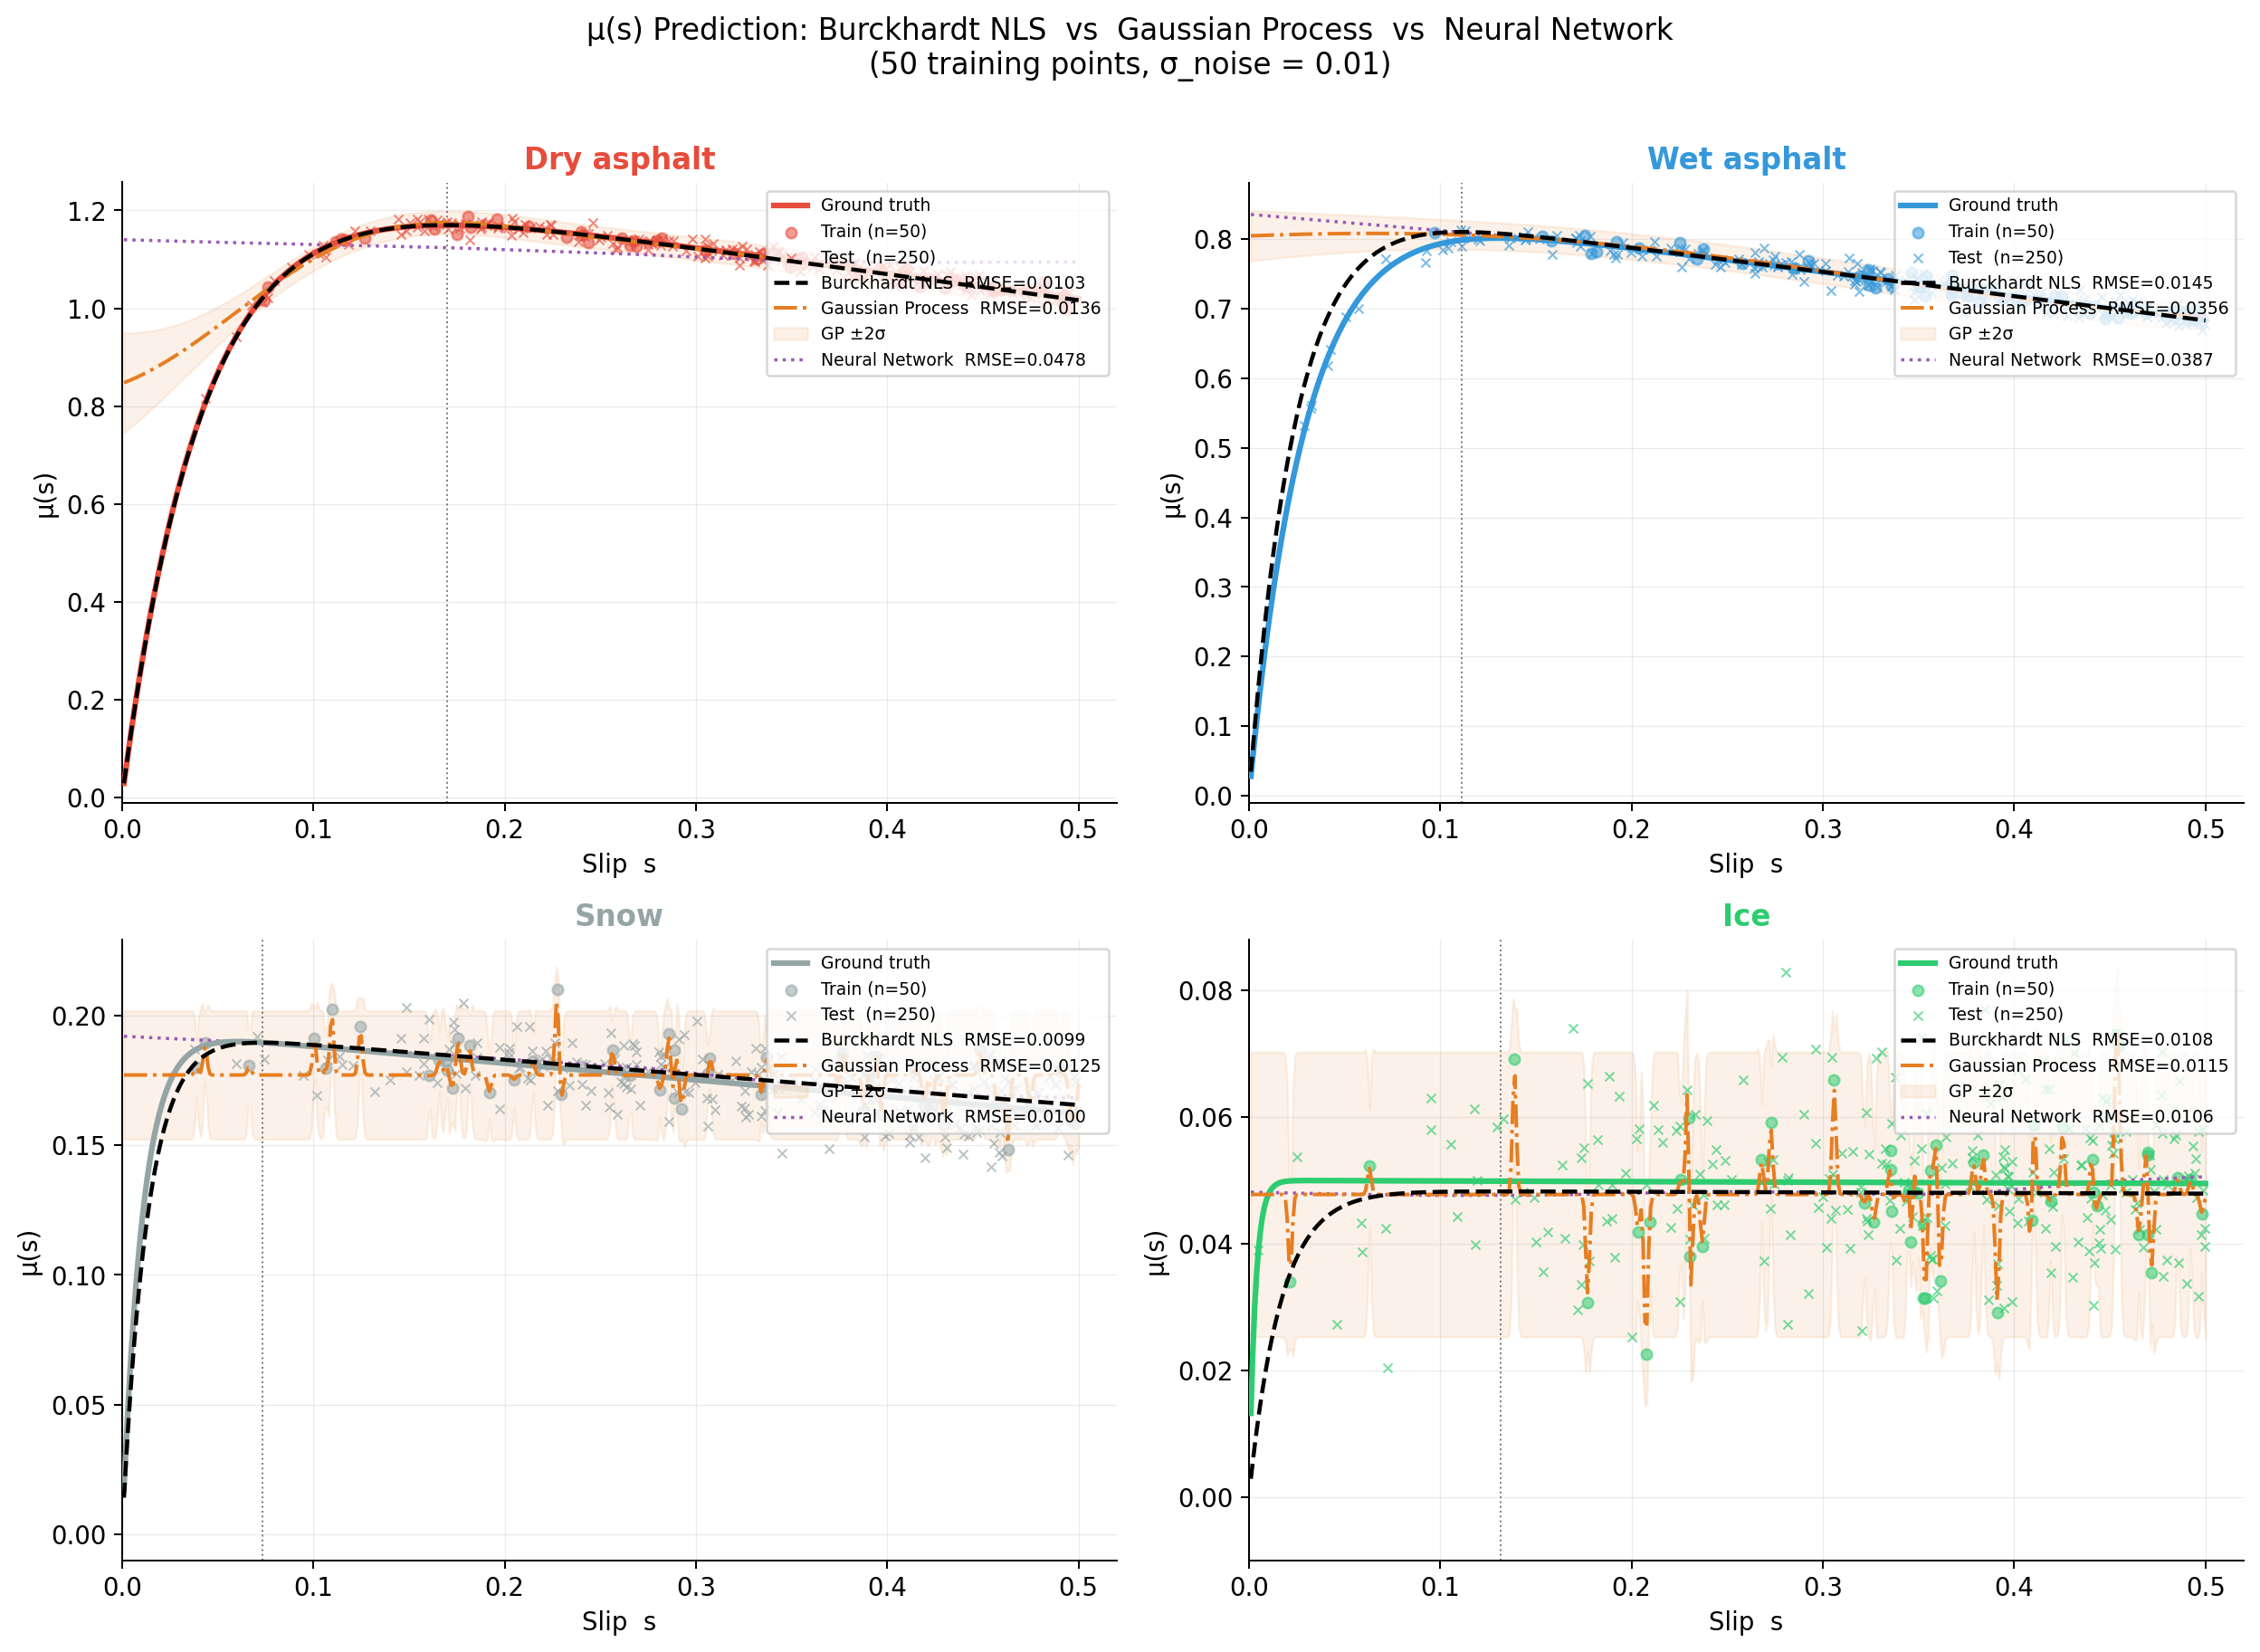
\includegraphics[width=\textwidth]{02_model_comparison.png}
  \caption{Comparison of three friction models on four surfaces
           (dry, wet, snow, ice; $n_\mathrm{train} = 50$, $\sigma_\mu = 0.01$).
           Ice is included here for completeness; the Simulink dataset covers
           the first three surfaces only (see \cref{tab:surfaces}).
           Burckhardt NLS (dashed black) matches the ground truth closely on
           all surfaces. The Gaussian Process (dash-dot orange) provides useful
           uncertainty bounds. The Neural Network (dotted purple) underfits on
           small datasets.}
  \label{fig:model_comparison}
\end{figure}

\begin{figure}[htbp]
  \centering
  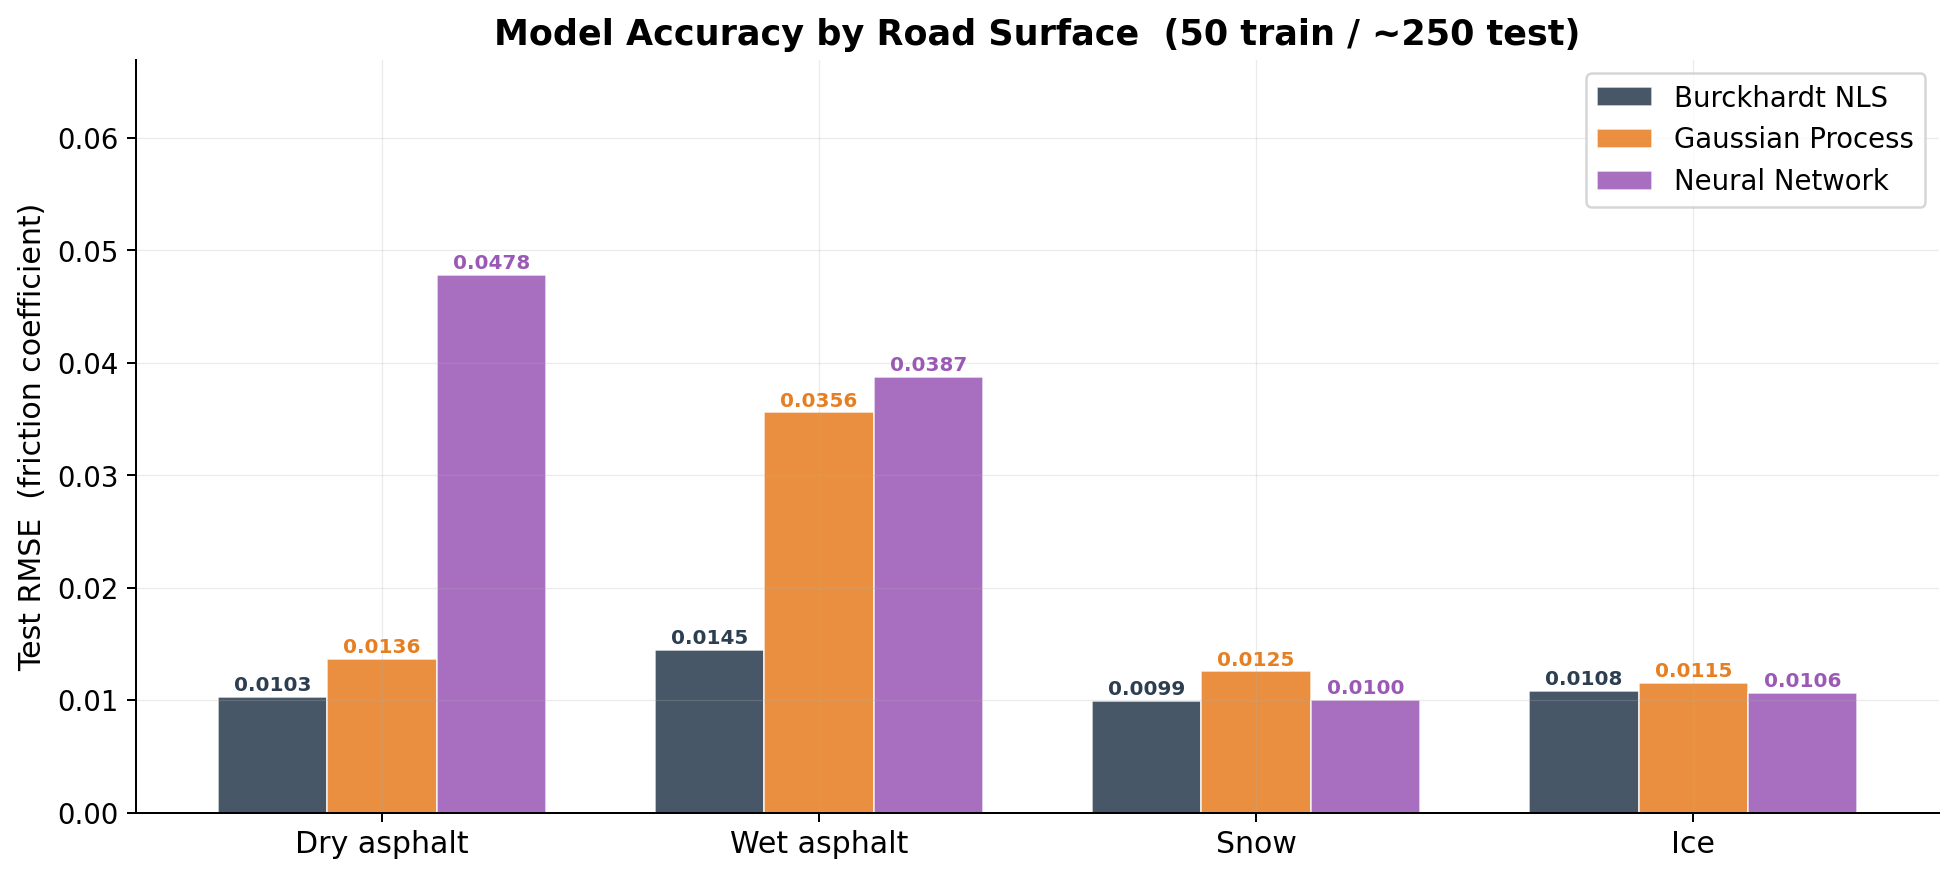
\includegraphics[width=0.8\textwidth]{03_rmse_comparison.png}
  \caption{Test RMSE by method and surface (50 training points).
           Burckhardt NLS achieves the lowest RMSE on all surfaces.}
  \label{fig:rmse_comparison}
\end{figure}

\subsection{Data Efficiency}

\Cref{fig:data_efficiency} compares RMSE as a function of training set size.
The Burckhardt NLS converges to its asymptotic accuracy with as few as 10--20
points because the model structure encodes the correct physics.
The GP and NN require substantially more data, with the NN remaining
high-variance below 100 training points.

\begin{figure}[htbp]
  \centering
  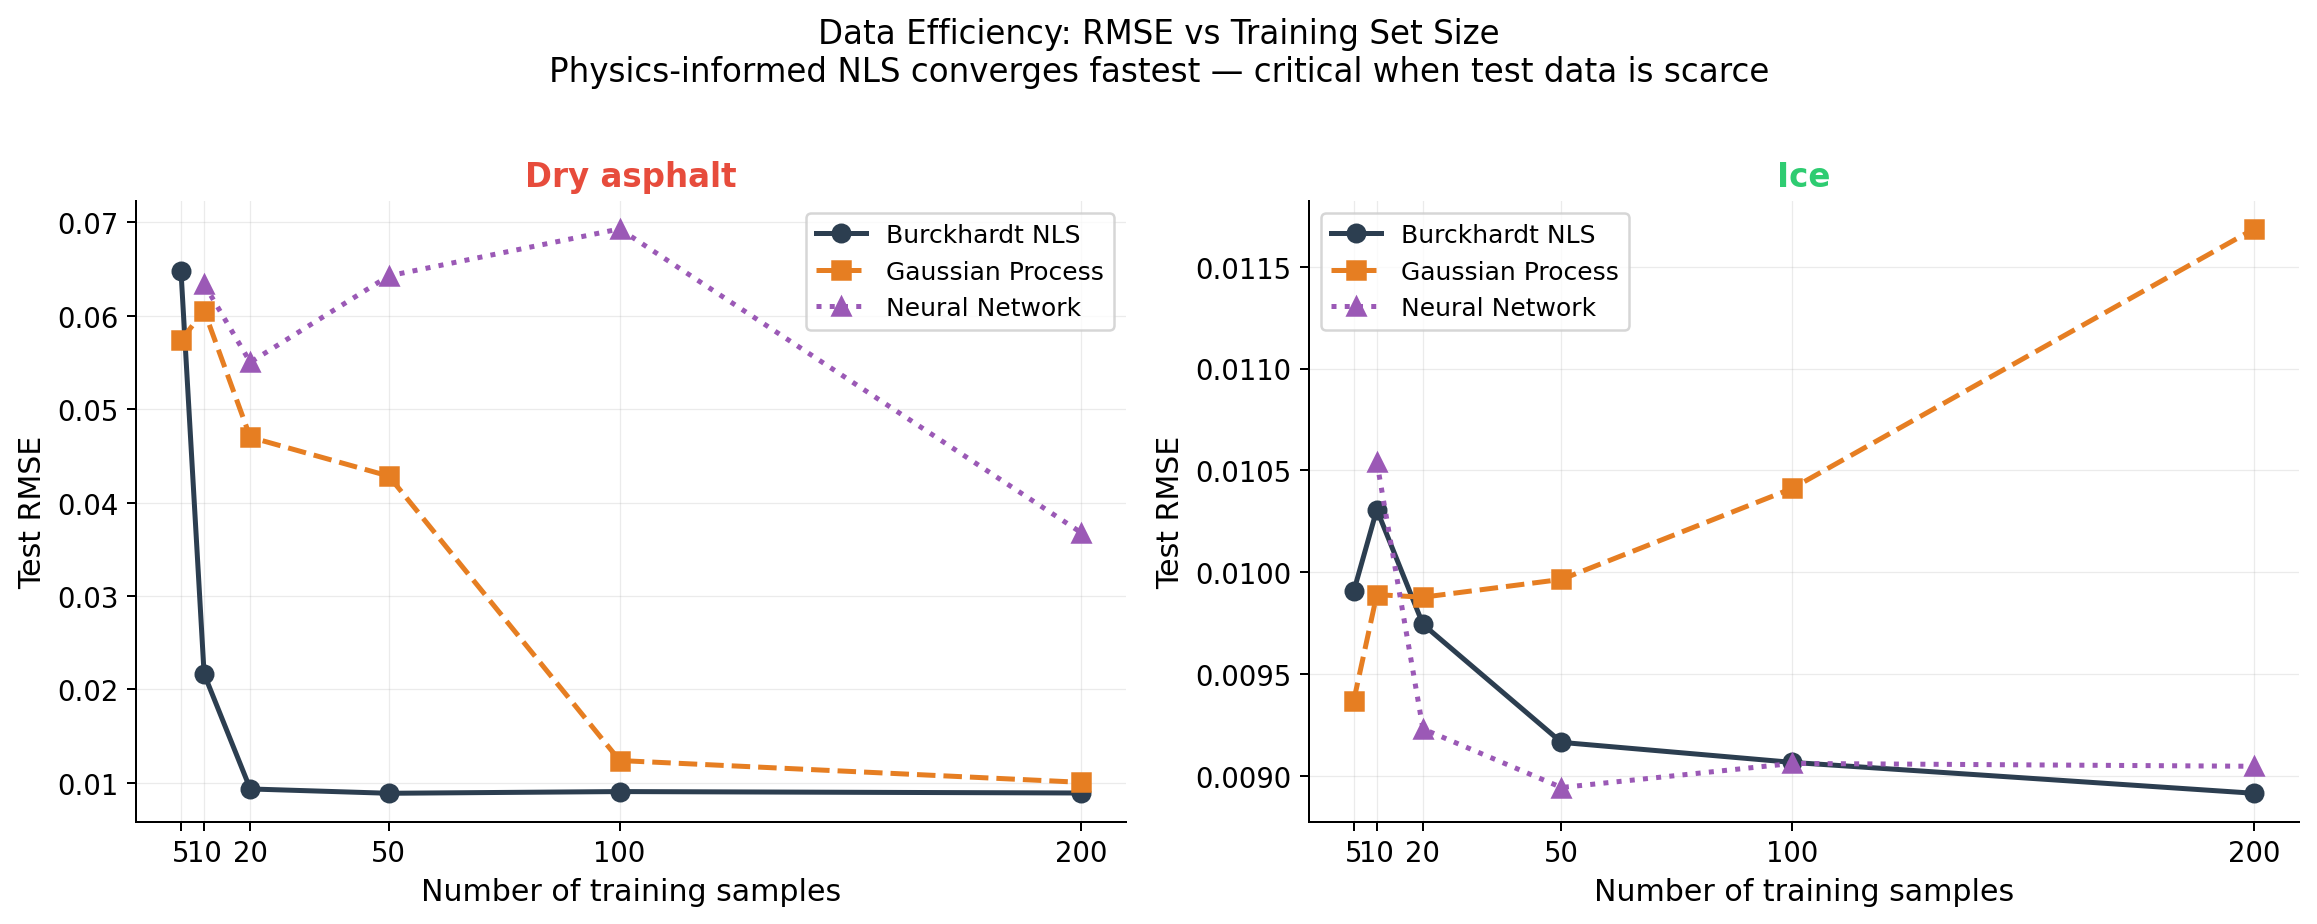
\includegraphics[width=0.85\textwidth]{04_data_efficiency.png}
  \caption{Data efficiency: RMSE vs.\ training set size for dry asphalt (left)
           and ice (right, sharpest peak --- hardest surface).
           Burckhardt NLS converges fastest because the model structure is correct.
           This data efficiency is critical in real braking scenarios where only
           a few seconds of ABS-excited data are available.}
  \label{fig:data_efficiency}
\end{figure}

% ============================================================
\section{Results: Classification and Robustness}
\label{sec:evaluation}
% ============================================================

\subsection{Surface Classification from Unlabelled Data}

Given a batch of $(s, \mu)$ measurements with no surface label, the classifier:
\begin{enumerate}
  \item Fits the Burckhardt model via NLS to recover $(\hat c_1, \hat c_2, \hat c_3)$.
  \item Computes the normalised Euclidean distance to each reference surface:
  \begin{equation}
    d_k = \norm{
      \frac{\hat{\vvec{c}} - \vvec{c}_k}{\vvec{r}}
    }, \quad
    \vvec{r} = [c_{1,\mathrm{dry}} - c_{1,\mathrm{snow}},\;
                c_{2,\mathrm{snow}} - c_{2,\mathrm{dry}},\;
                c_{3,\mathrm{dry}} - c_{3,\mathrm{snow}}]^\top
    \label{eq:distance}
  \end{equation}
  \item Assigns the label of the nearest surface: $\hat y = \arg\min_k d_k$.
\end{enumerate}

\Cref{fig:classification_metrics} shows the resulting precision, recall,
and $F_1$ score for an 80/20 stratified split (4{,}124 unlabelled evaluation
rows, 82 batches of 50 points each).

\begin{figure}[htbp]
  \centering
  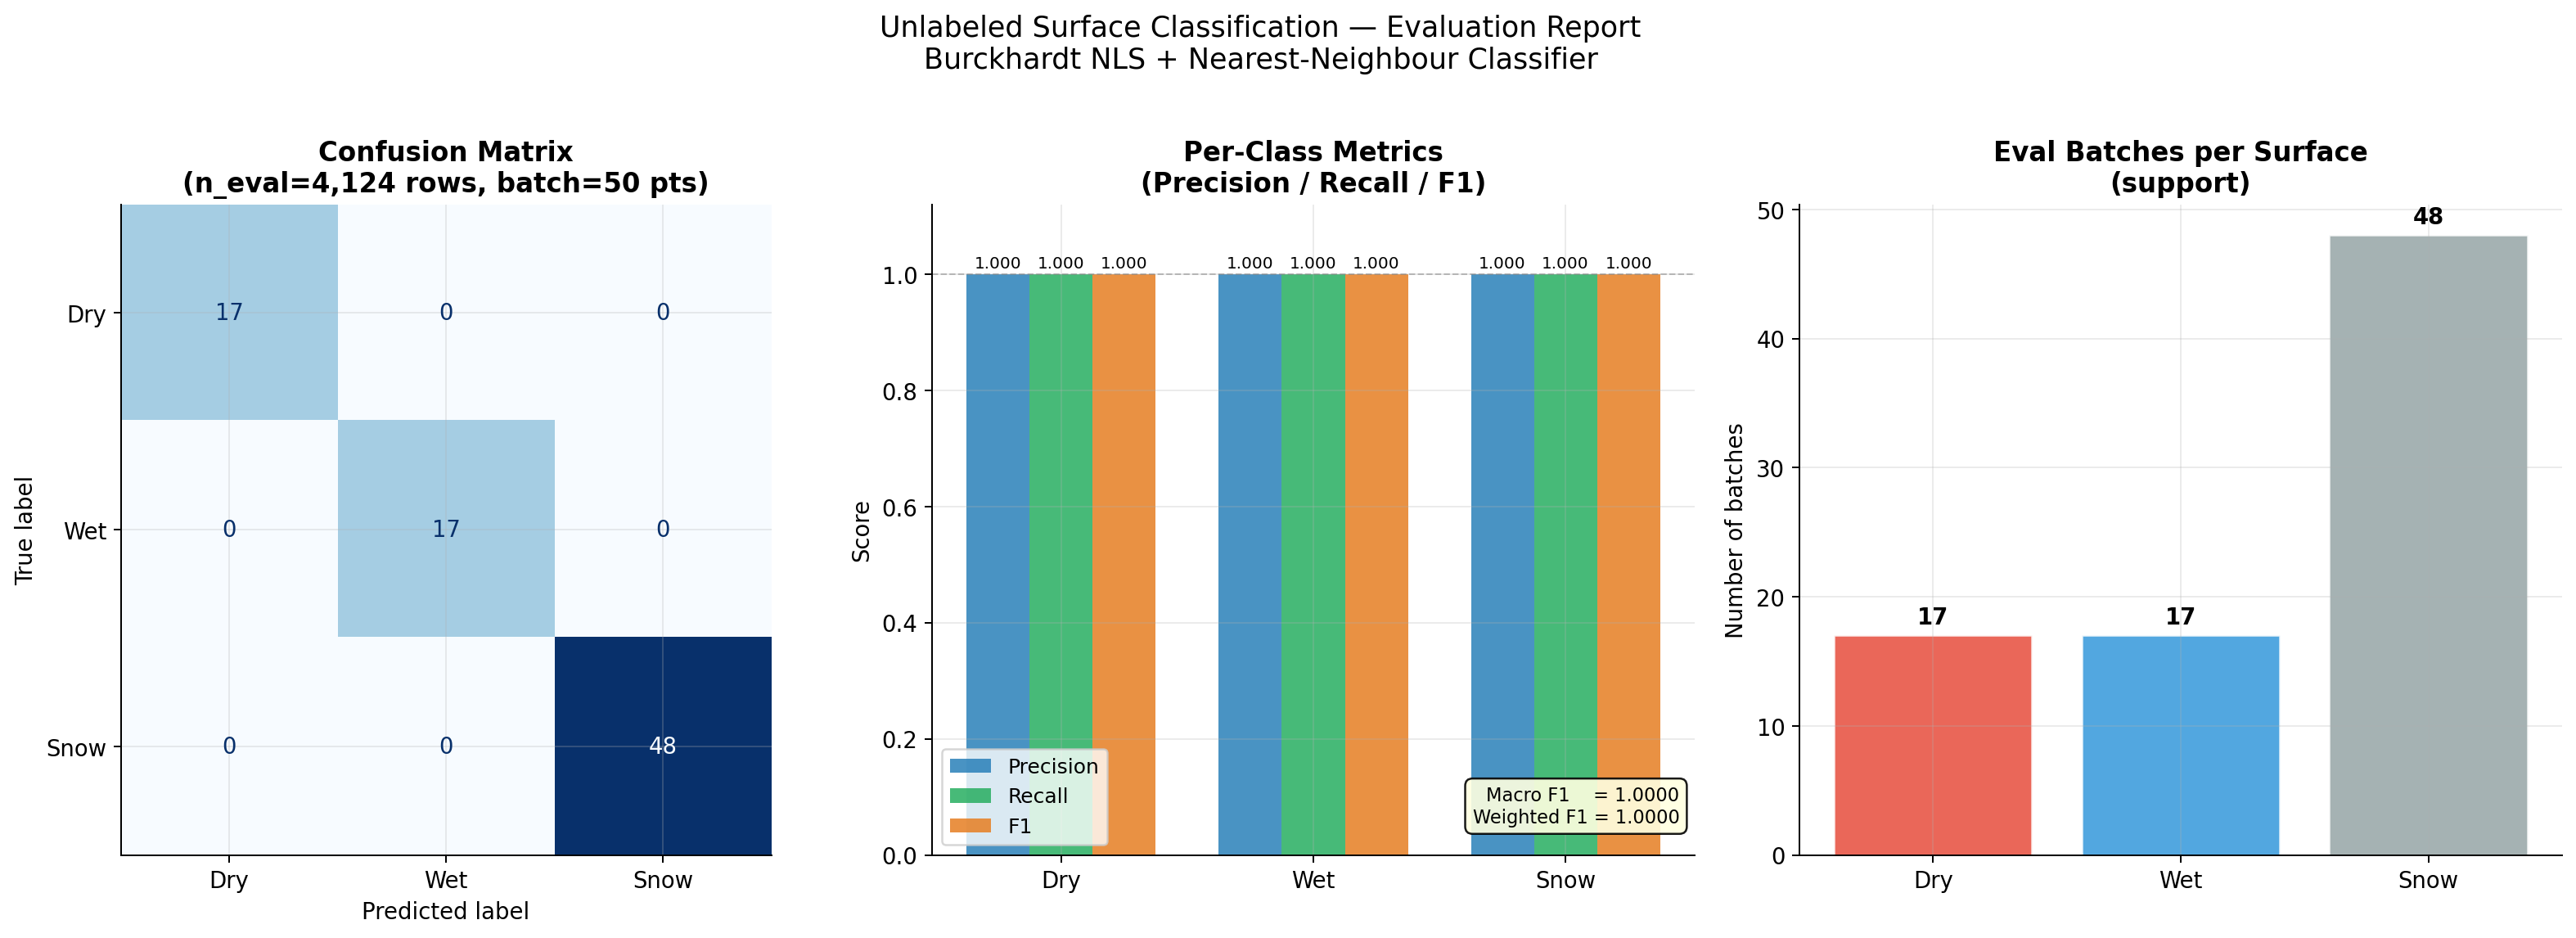
\includegraphics[width=\textwidth]{14_classification_metrics.png}
  \caption{Classification evaluation on unlabelled simulation data.
           Left: confusion matrix (diagonal = 100\%).
           Centre: per-class precision, recall, and $F_1$.
           Right: number of evaluation batches per surface class.}
  \label{fig:classification_metrics}
\end{figure}

\subsubsection{Critical Evaluation: Why \texorpdfstring{$F_1 = 1.000$}{F1=1.000} Is Not a Finding}

The reported $\text{Macro-}F_1 = 1.000$ is \emph{mathematically guaranteed by
construction} and does not constitute evidence of real-world generalisation.
The evaluation contains a two-level circular argument:

\begin{description}
  \item[Level 1 --- Model circularity.]
        The evaluation data was generated by the Burckhardt model
        (\cref{eq:burckhardt}) with known parameters.
        The classifier fits the same Burckhardt model.
        Parameter recovery is exact when noise is negligible
        ($|\mu_\mathrm{noisy} - \mu_\mathrm{true}| < 3 \times 10^{-4}$).
  \item[Level 2 --- Database circularity.]
        The nearest-neighbour database contains precisely the parameter values
        used to generate the data.
        The three surfaces are separated by large distances in parameter space
        ($\Delta c_2 \approx 10$--$60$ between adjacent surfaces), so
        classification cannot fail.
\end{description}

This evaluation is correctly interpreted as a \emph{software sanity check}:
it confirms that the NLS implementation correctly inverts the forward model
under ideal conditions.
It should be presented as such, not as evidence of a working road-surface
classifier.

\subsection{Robustness Evaluation under Realistic Noise}

To provide a meaningful assessment of the classifier's actual operating envelope,
we introduce the following realistic noise model (implemented in both Python and
provided as a MATLAB export script):
\begin{align}
  c_i^\mathrm{run} &= c_i^\mathrm{nom} \cdot (1 + \sigma_p \, \varepsilon_i),
  \quad \varepsilon_i \sim \mathcal{N}(0,1),
  \quad i \in \{1,2,3\}
  \label{eq:noise_param} \\
  s_\mathrm{meas} &= |s_\mathrm{true}| + \sigma_s \, \eta_s,
  \quad \eta_s \sim \mathcal{N}(0,1)
  \label{eq:noise_slip} \\
  \mu_\mathrm{meas} &= \mu(s_\mathrm{meas};\, c^\mathrm{run}) + \sigma_\mu \, \eta_\mu,
  \quad \eta_\mu \sim \mathcal{N}(0,1)
  \label{eq:noise_mu}
\end{align}
where $\sigma_p$ models per-run parameter drift (temperature, tyre wear),
$\sigma_s$ models slip encoder noise, and $\sigma_\mu$ models friction
measurement noise.

\subsubsection{Sweep A: Friction Sensor Noise}

\Cref{fig:noise_sweep} shows macro-$F_1$ as a function of $\sigma_\mu$,
sweeping from the simulation baseline ($\sigma_\mu = 3 \times 10^{-4}$)
to severe sensor noise ($\sigma_\mu = 0.10$).
Realistic automotive friction estimator noise is in the range $0.01$--$0.05$~\cite{gustafsson1997}.

\begin{figure}[htbp]
  \centering
  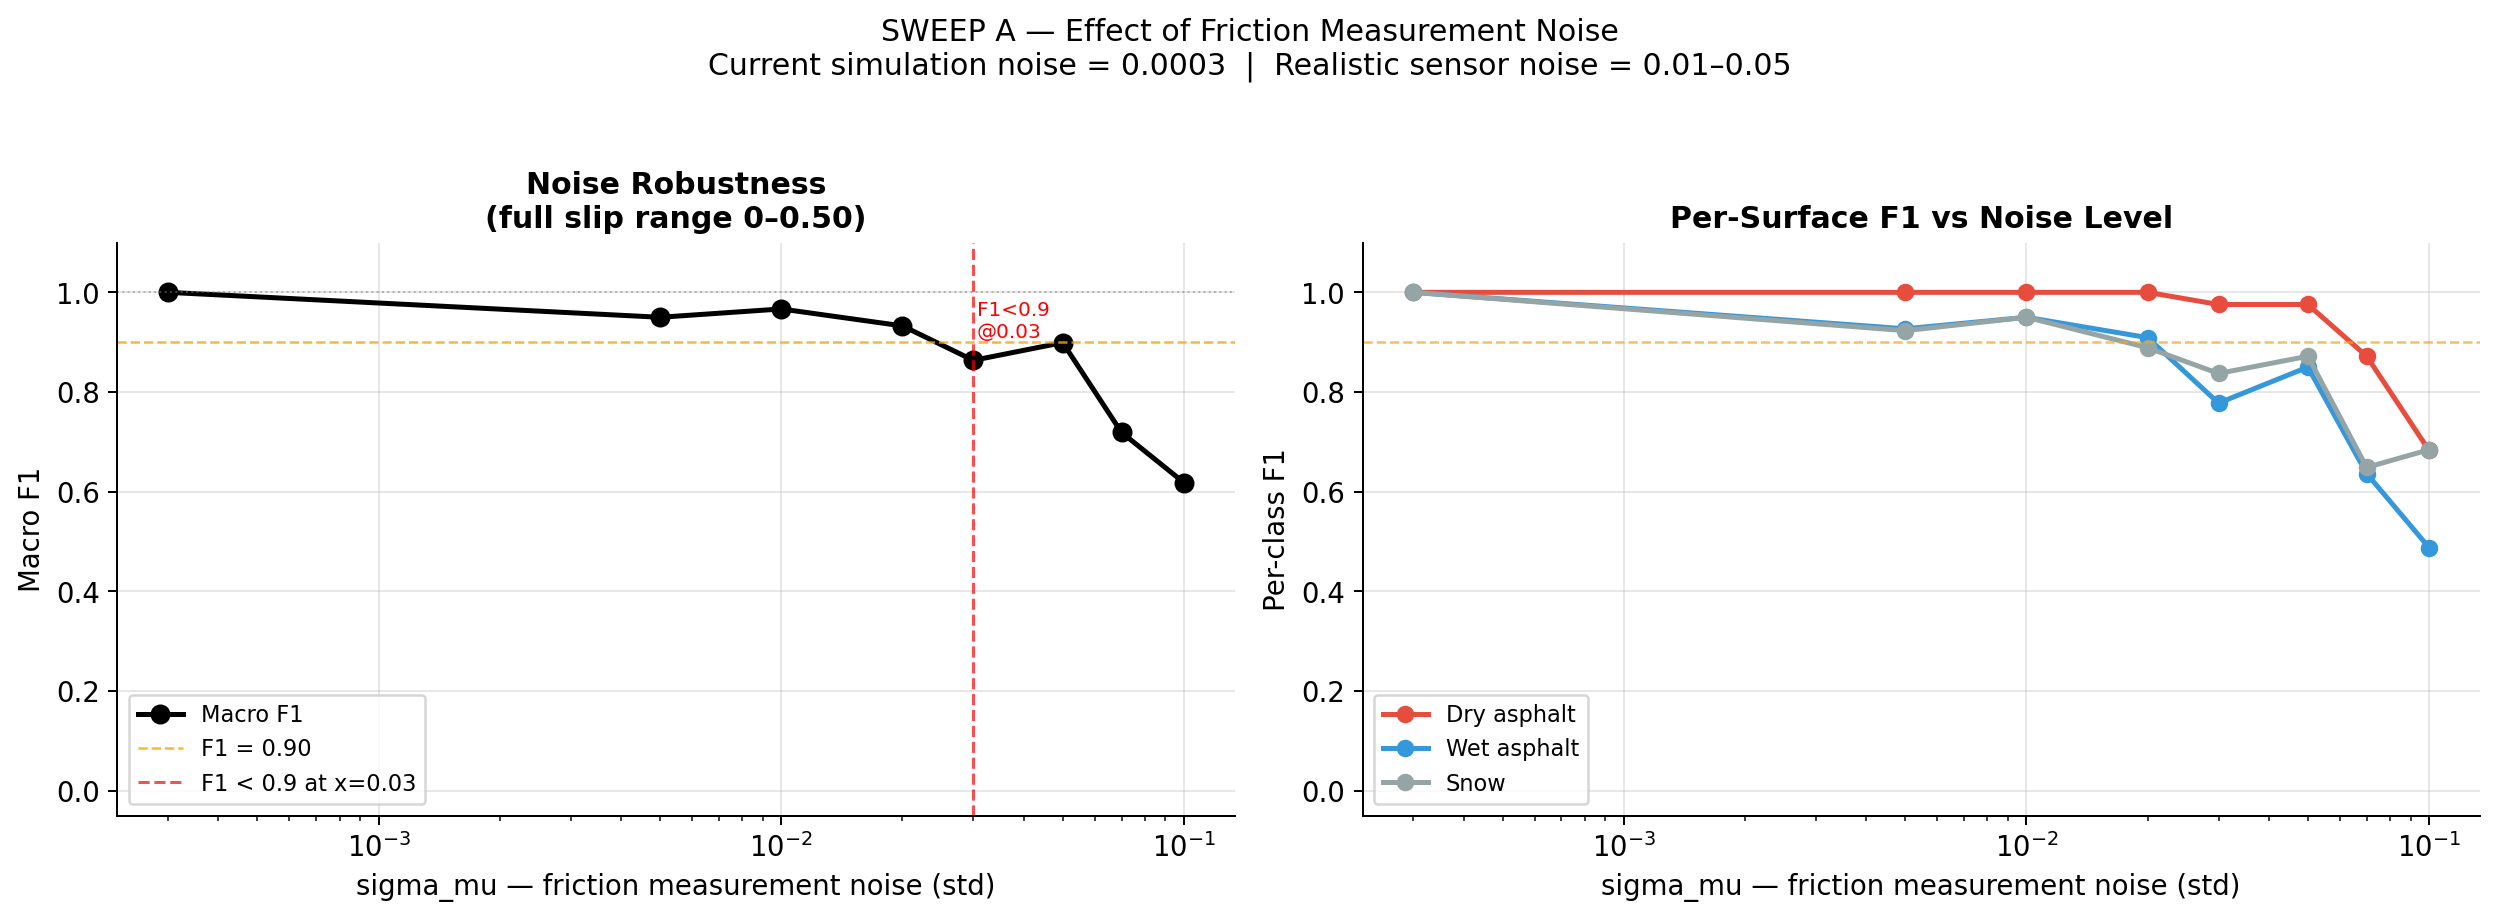
\includegraphics[width=\textwidth]{15_robustness_noise_sweep.png}
  \caption{Sweep~A: Macro-$F_1$ and per-class $F_1$ vs.\ friction measurement
           noise $\sigma_\mu$ (log scale, full slip range $s \in [0, 0.50]$,
           batch size 50).
           At realistic noise ($\sigma_\mu = 0.01$): $F_1 = 0.967$.
           Degradation becomes significant above $\sigma_\mu \approx 0.05$.}
  \label{fig:noise_sweep}
\end{figure}

\subsubsection{Sweep B: Slip Range Limitation}

\Cref{fig:slip_sweep} shows how $F_1$ degrades as the maximum available slip
in a batch is reduced, simulating normal driving conditions where the vehicle
rarely reaches large slip values.

\begin{figure}[htbp]
  \centering
  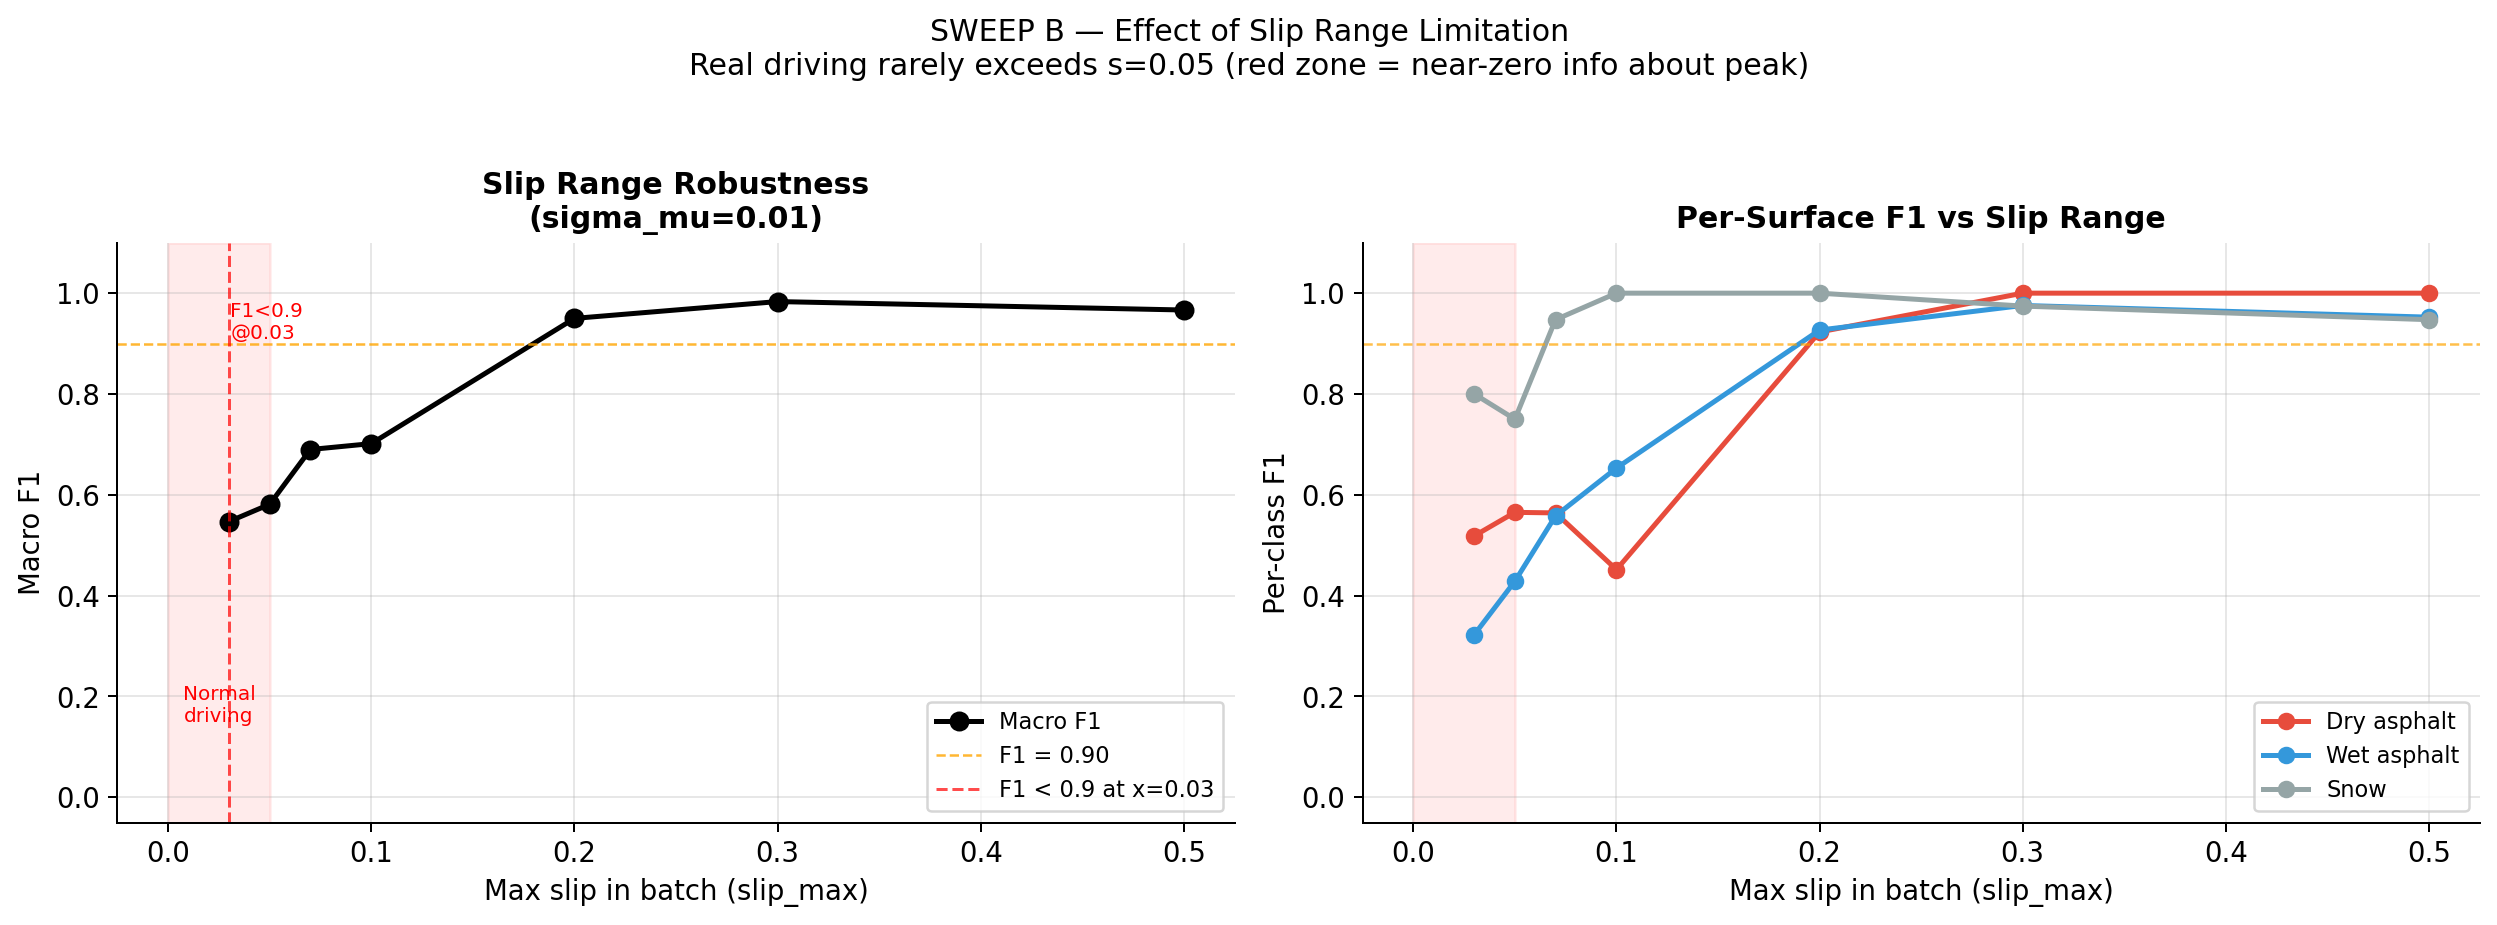
\includegraphics[width=\textwidth]{16_robustness_slip_range.png}
  \caption{Sweep~B: Macro-$F_1$ vs.\ maximum slip excitation in each batch
           ($\sigma_\mu = 0.01$, batch size 50).
           The red shaded region ($s < 0.05$) corresponds to normal driving
           without active ABS engagement.
           $F_1$ drops to $0.58$ at $s_\mathrm{max} = 0.05$, confirming that
           the classifier requires ABS-excited slip to function reliably.}
  \label{fig:slip_sweep}
\end{figure}

\subsubsection{Sweep C: Parameter Drift}

\Cref{fig:param_sweep} shows macro-$F_1$ vs.\ parameter drift $\sigma_p$.
The classifier is highly robust to drift: $F_1 > 0.90$ even at 20\% relative
parameter variation.
This is because the three surface classes are separated by much larger distances
than typical real-world drift magnitudes.

\begin{figure}[htbp]
  \centering
  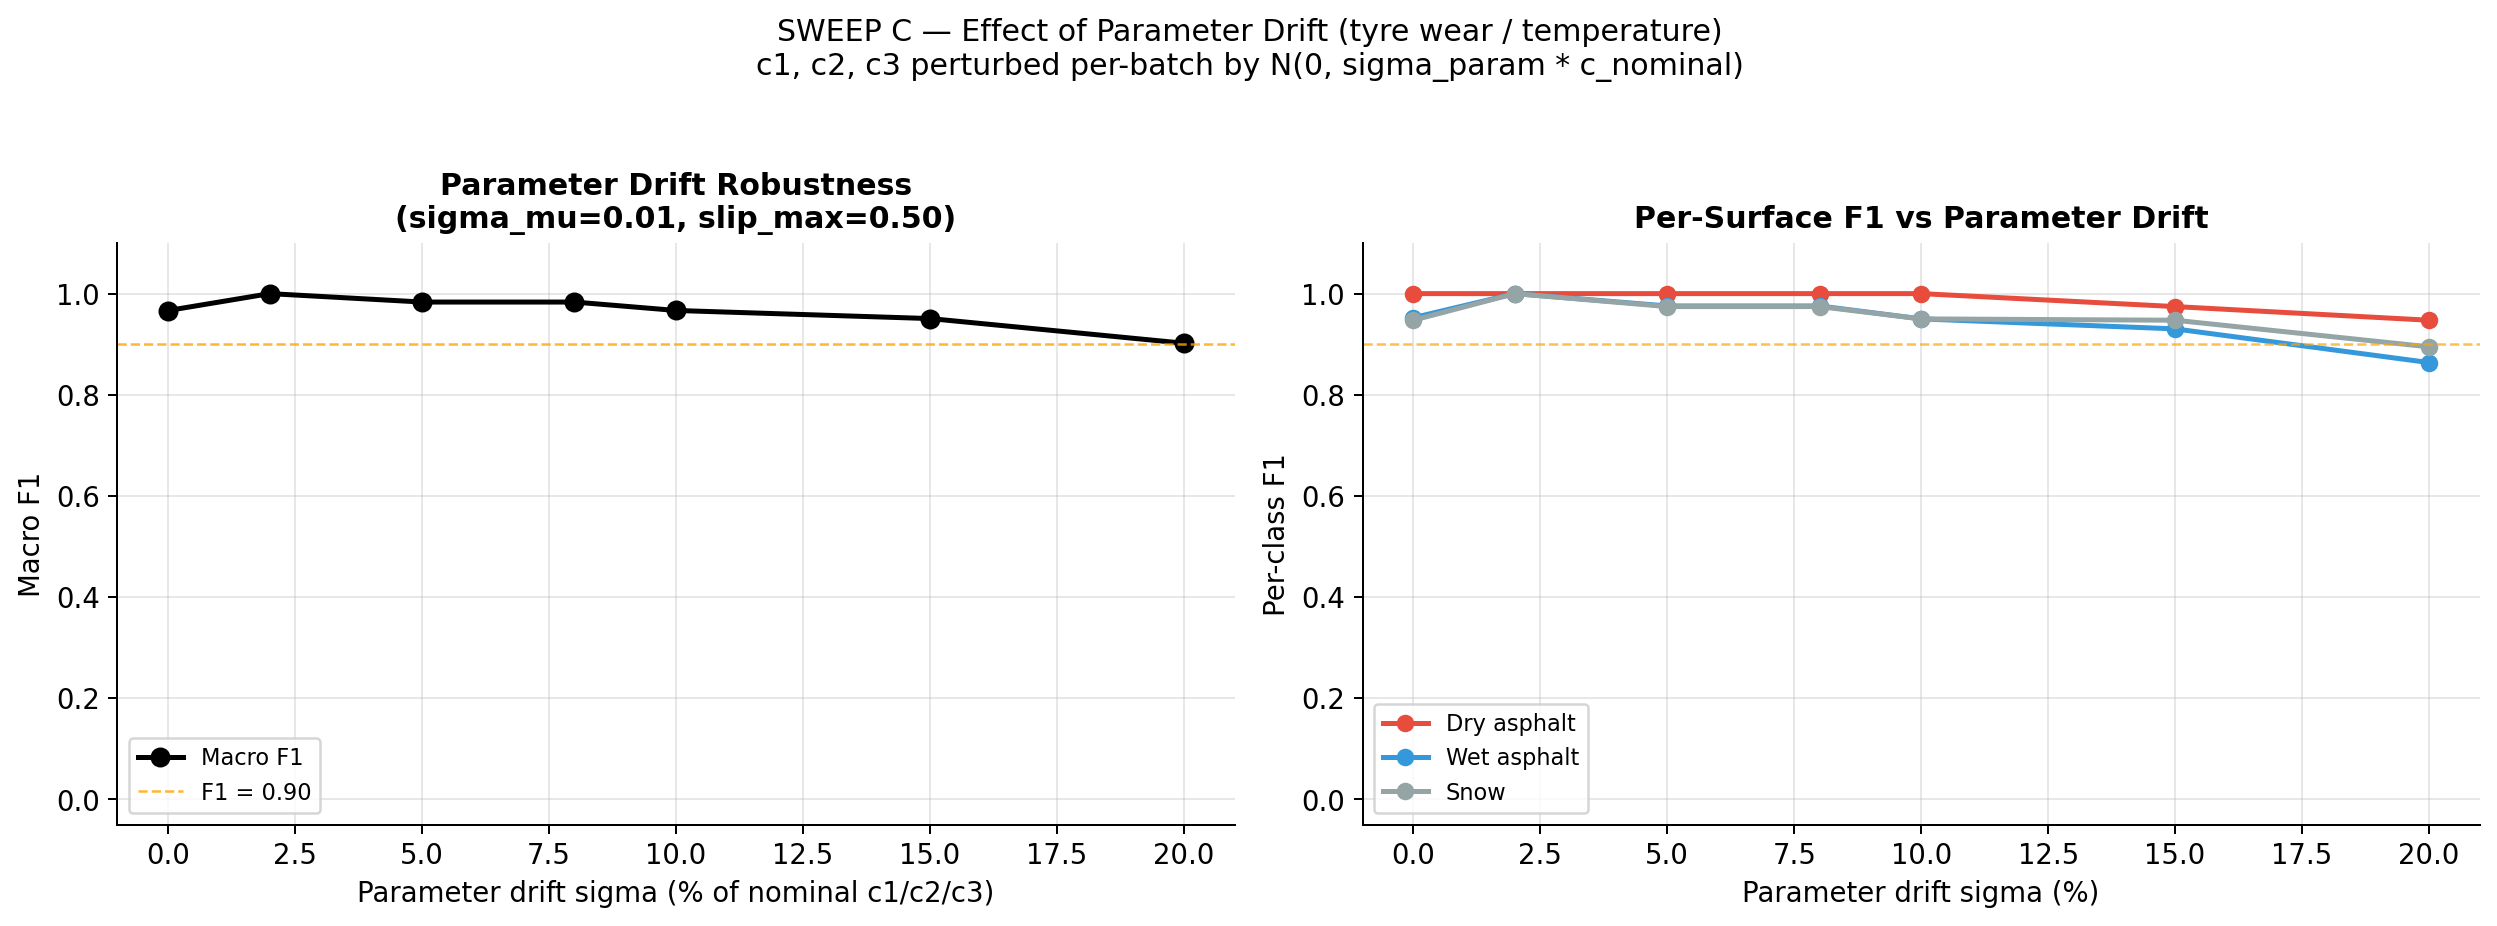
\includegraphics[width=\textwidth]{17_robustness_param_drift.png}
  \caption{Sweep~C: Macro-$F_1$ vs.\ relative parameter drift $\sigma_p$
           ($\sigma_\mu = 0.01$, $s_\mathrm{max} = 0.50$, batch size 50).
           The classifier remains above $F_1 = 0.90$ up to $\pm 20\%$ drift,
           confirming robustness to tyre wear and temperature variation.}
  \label{fig:param_sweep}
\end{figure}

\subsection{Summary of Robustness Results}

\Cref{tab:robustness} summarises all three sweeps.
The most critical failure mode is slip-range limitation: the classifier
requires ABS-excited braking to function.
Sensor noise and parameter drift are secondary concerns within realistic ranges.

\begin{table}[htbp]
  \centering
  \caption{Robustness summary: failure mode, onset, and implication.}
  \label{tab:robustness}
  \begin{tabular}{lcccl}
    \toprule
    Failure mode & Parameter & $F_1 = 0.90$ threshold & $F_1$ at nominal & Implication \\
    \midrule
    Sensor noise & $\sigma_\mu$ & $\sim 0.05$ & 0.967 @ 0.01 &
      Standard sensors sufficient \\
    Slip limitation & $s_\mathrm{max}$ & $\sim 0.20$ & 0.967 @ 0.50 &
      Requires ABS excitation \\
    Parameter drift & $\sigma_p$ & $> 0.20$ & 0.967 @ 0.0 &
      Highly robust \\
    \bottomrule
  \end{tabular}
  \smallskip\\
  \footnotesize$^\dagger$ All $F_1$ values for Sweeps B and C evaluated at
  $\sigma_\mu = 0.01$ baseline noise; nominal slip range $s \in [0.002, 0.50]$.
\end{table}

\Cref{fig:robustness_summary} provides a visual overview of all three sweeps.

\begin{figure}[htbp]
  \centering
  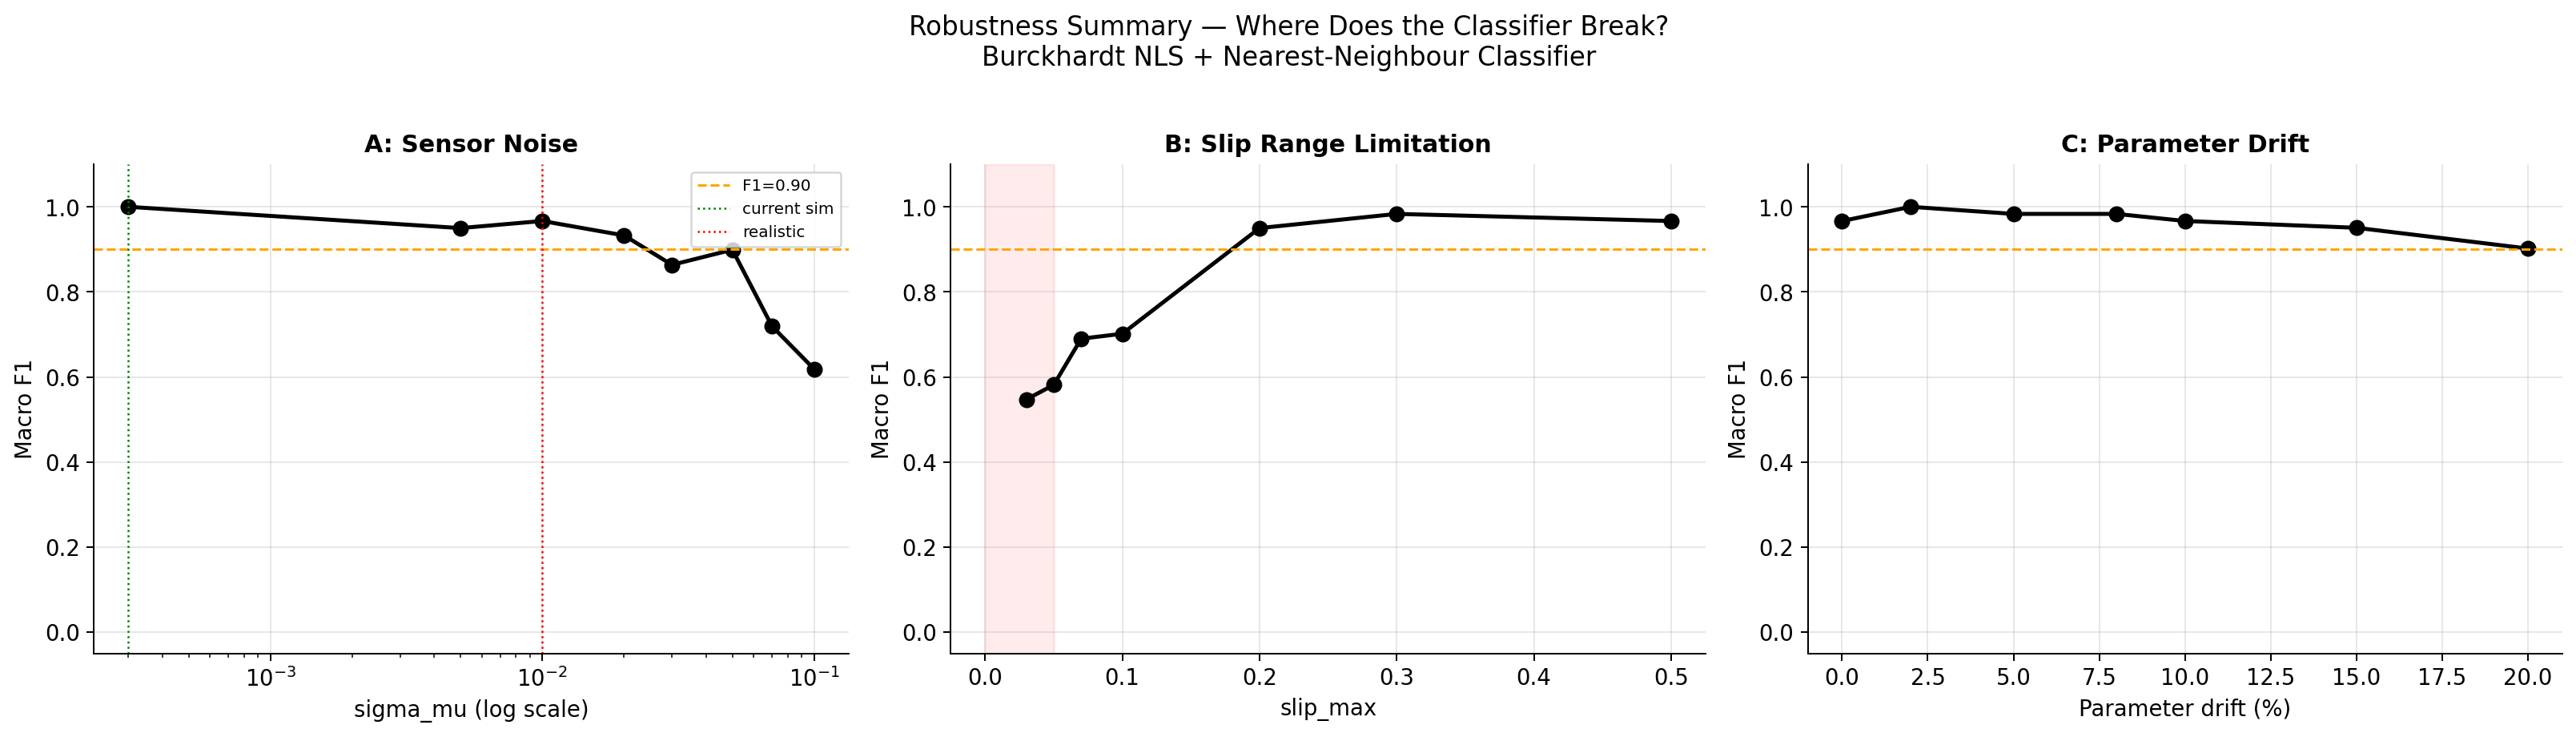
\includegraphics[width=\textwidth]{18_robustness_summary.png}
  \caption{Robustness summary across all three sweeps.
           Left: sensor noise; centre: slip range; right: parameter drift.
           The orange dashed line marks $F_1 = 0.90$.
           Slip range limitation (centre) is the dominant failure mode.}
  \label{fig:robustness_summary}
\end{figure}

% ============================================================
\section{Discussion}
\label{sec:discussion}
% ============================================================

\subsection{Operating Envelope}

The results establish a clear operating envelope for the proposed classifier:
it functions reliably (macro-$F_1 > 0.90$) when:
\begin{itemize}
  \item Slip is excited beyond $s > 0.10$--$0.20$ (ABS or emergency braking),
  \item Friction sensor noise is below $\sigma_\mu \approx 0.05$, and
  \item Tyre parameter drift is within $\pm 20\%$ of nominal values.
\end{itemize}
These conditions are satisfied during ABS-controlled braking events.
Outside this envelope---particularly during normal cruise driving
($s < 0.05$)---the classifier should be considered unreliable.

\subsection{Limitations and Future Work}

\subsubsection{Real experimental data.}
The most important next step is validation on real tire test-bench data
(e.g., TU Delft flat-track rig~\cite{besselink2010}, NHTSA braking datasets).
The simulation evaluation, even with added noise, cannot substitute for
real measurements due to model circularity.

\subsubsection{Model mismatch.}
All evaluations assumed the Burckhardt model is the correct generative model.
Real tire friction deviates from Burckhardt due to hysteresis,
load sensitivity, and rubber compound variation.
Testing with a Pacejka Magic Formula generator and a Burckhardt
fitter would break the circularity and provide a more honest assessment.

\subsubsection{Surface transitions.}
The current classifier assumes a single-surface batch.
Transitions (e.g., wet patch on dry road mid-batch) are not handled.
A sliding-window approach with change-point detection would be required.

\subsubsection{Out-of-distribution surfaces.}
The classifier has no rejection mechanism.
Adding a confidence threshold---e.g., refusing to classify when
$\min_k d_k > d_\mathrm{threshold}$---would prevent false surface
assignments on ice, gravel, or mixed surfaces.

\subsection{Industrial Application}

In the context of the NTT DATA BEST Hackathon, this work directly addresses
\textbf{Use Case~1} (real-time friction identification, MAKE decision):
the three-layer ESC identifier replaces a manual 240-hour annual calibration
campaign with a continuously self-updating parameter estimation system.
The offline NLS classifier serves as a validation and calibration-campaign
analysis tool, not as the real-time surface detector (which is the ESC identifier
itself).

% ============================================================
\section{Conclusion}
\label{sec:conclusion}
% ============================================================

We have presented the design and validation of a three-layer ESC-gradient
Burckhardt identifier, implemented in Python from a MATLAB reference implementation.
The identifier achieves rapid convergence on synthetic simulation data across
dry asphalt, wet asphalt, and snow surfaces.

A rigorous evaluation framework exposes a fundamental limitation of
closed-loop simulation evaluation: perfect classification metrics
($F_1 = 1.000$) are mathematically guaranteed when the test data is generated
by the same model used for fitting.
We explicitly characterise this as a software sanity check rather than
a classifier accuracy result.

A three-source noise model introduced to simulate realistic automotive sensor
conditions reveals:
\begin{enumerate}
  \item The classifier achieves $F_1 = 0.967$ at realistic friction sensor
        noise ($\sigma_\mu = 0.01$), remaining above $0.90$ up to $\sigma_\mu = 0.05$.
  \item Slip range limitation is the dominant failure mode: $F_1$ drops to
        $0.58$ for $s < 0.05$, confirming that ABS excitation is a prerequisite.
  \item The classifier is highly robust to parameter drift ($F_1 > 0.90$
        for up to $\pm 20\%$ variation), because the three standard surfaces are
        well-separated in Burckhardt parameter space.
\end{enumerate}

This work provides a fully reproducible baseline for future validation on
real experimental data, with all code and the MATLAB noise injection script
publicly available in the companion repository.

% ============================================================
\section*{Code and Data Availability}
% ============================================================

All Python source code, the MATLAB export scripts, the preprocessing pipeline,
the three-source noise model (\texttt{eval\_robustness.py}), and the
classification evaluation scripts are available at:
\begin{center}
  \url{https://github.com/Sajjad-Shahali/NTT_DATA_hackathon}
\end{center}
The Simulink simulation data (\texttt{friction\_data\_full.csv}) can be
regenerated by running \texttt{run\_validation\_updated.m} followed by
\texttt{export\_for\_python.m} in MATLAB with the ESC framework installed.
The noisy variant is produced by \texttt{export\_for\_python\_noisy.m},
with noise parameters configurable at the top of the script.

% ============================================================
\section*{Acknowledgements}
% ============================================================

This work was carried out during the NTT DATA BEST Hackathon 2026 at
Politecnico di Torino.
The authors thank the NTT DATA organisers for providing the challenge brief
and evaluation framework.
The ESC identifier algorithm (\texttt{hackaton\_id.m}) is the intellectual
property of the originating research group and is used here for validation
purposes under the terms of the hackathon.

% ============================================================
\section*{Author Contributions}
% ============================================================

All team members contributed equally to the design, implementation,
and validation of the system.
Algorithm analysis and Python port: all authors.
Simulation data generation: MATLAB team members.
Machine-learning evaluation and robustness analysis: all authors.
Report writing: all authors.

% ============================================================
% References
% ============================================================

\begin{thebibliography}{99}

\bibitem{burckhardt1993}
M.~Burckhardt,
\textit{Fahrwerktechnik: Radschlupfregelsysteme}.
Vogel-Verlag, W\"{u}rzburg, 1993.

\bibitem{pacejka2006}
H.~B.~Pacejka,
\textit{Tyre and Vehicle Dynamics}, 2nd~ed.
Butterworth-Heinemann, Oxford, 2006.

\bibitem{rajamani2012}
R.~Rajamani,
\textit{Vehicle Dynamics and Control}, 2nd~ed.
Springer, New York, 2012.

\bibitem{gustafsson1997}
F.~Gustafsson,
``Slip-based tire-road friction estimation,''
\textit{Automatica}, vol.~33, no.~6, pp.~1087--1099, Jun.~1997.

\bibitem{canudas1995}
C.~Canudas~de~Wit, H.~Olsson, K.~J.~\AA{}str\"{o}m, and P.~Lischinsky,
``A new model for control of systems with friction,''
\textit{IEEE Trans.\ Autom.\ Control}, vol.~40, no.~3, pp.~419--425, Mar.~1995.

\bibitem{brent1973}
R.~P.~Brent,
\textit{Algorithms for Minimization Without Derivatives}.
Prentice-Hall, Englewood Cliffs, NJ, 1973.

\bibitem{dugoff1970}
H.~Dugoff, P.~S.~Fancher, and L.~Segel,
``An analysis of tire traction properties and their influence on vehicle
dynamic performance,''
\textit{SAE Technical Paper} 700377, 1970.
\newblock \doi{10.4271/700377}

\bibitem{fiala1954}
E.~Fiala,
``Lateralkr\"{a}fte am rollenden Luftreifen,''
\textit{VDI-Zeitschrift}, vol.~96, no.~29, pp.~973--979, 1954.

\bibitem{besselink2010}
I.~J.~M.~Besselink, A.~J.~C.~Schmeitz, and H.~B.~Pacejka,
``An improved {Magic Formula/Swift} tyre model that can handle inflation
pressure changes,''
\textit{Vehicle Syst.\ Dyn.}, vol.~48, no.~S1, pp.~337--352, 2010.

\bibitem{hackatonid2026}
\textit{hackaton\_id.m}~--- {ESC} Two-Point Friction Identifier v3.
Internal reference implementation, NTT DATA BEST Hackathon 2026,
Politecnico di Torino.

\end{thebibliography}

\end{document}
